\documentclass[12pt]{article}

\usepackage{amsmath, mathtools}
\usepackage{amsfonts}
\usepackage{amssymb}
\usepackage{graphicx}
\usepackage{colortbl}
\usepackage{xr}
\usepackage{longtable}
\usepackage{xfrac}
\usepackage{siunitx}
\usepackage{tabularx}
\usepackage{float}
\usepackage{booktabs}
\usepackage{caption}
\usepackage{pdflscape}
\usepackage{afterpage}
\usepackage{calc}
\usepackage{multirow}
\usepackage{array}
\usepackage{longtable}
\usepackage{rotating}
\usepackage{leftindex}

\usepackage[a4paper, total={7in, 9in}]{geometry}
\usepackage[acronym,nomain,section=subsection,numberedsection]{glossaries}
\usepackage[round]{natbib}
\usepackage[bookmarks=true,breaklinks]{hyperref}

%% Comments

\usepackage{color}

\newif\ifcomments\commentstrue %displays comments
%\newif\ifcomments\commentsfalse %so that comments do not display

\ifcomments
\newcommand{\authornote}[3]{\textcolor{#1}{[#3 ---#2]}}
\newcommand{\todo}[1]{\textcolor{red}{[TODO: #1]}}
\else
\newcommand{\authornote}[3]{}
\newcommand{\todo}[1]{}
\fi

\newcommand{\wss}[1]{\authornote{blue}{SS}{#1}} 
\newcommand{\plt}[1]{\authornote{magenta}{TPLT}{#1}} %For explanation of the template
\newcommand{\an}[1]{\authornote{cyan}{Author}{#1}}

%% Common Parts

\newcommand{\progname}{MECHTRON 4TB6} % PUT YOUR PROGRAM NAME HERE
\newcommand{\authname}{Group 1, UWheeledChair,
\\ Lisa Ji
\\ Haoyu Lin
\\ Yuntian Wang
\\ Zichun Yan } % AUTHOR NAMES                  

\usepackage{hyperref}
    \hypersetup{colorlinks=true, linkcolor=blue, citecolor=blue, filecolor=blue,
                urlcolor=blue, unicode=false}
    \urlstyle{same}
% \hypersetup{
%     colorlinks=true,       % false: boxed links; true: colored links
%     linkcolor=red,          % color of internal links (change box color with linkbordercolor)
%     citecolor=green,        % color of links to bibliography
%     filecolor=magenta,      % color of file links
%     urlcolor=cyan           % color of external links
% }

% For easy change of table widths
\newcommand{\colZwidth}{1.0\textwidth}
\newcommand{\colAwidth}{0.13\textwidth}
\newcommand{\colBwidth}{0.82\textwidth}
\newcommand{\colCwidth}{0.1\textwidth}
\newcommand{\colDwidth}{0.05\textwidth}
\newcommand{\colEwidth}{0.8\textwidth}
\newcommand{\colFwidth}{0.17\textwidth}
\newcommand{\colGwidth}{0.5\textwidth}
\newcommand{\colHwidth}{0.28\textwidth}

\makenoidxglossaries
    \newlength\maxlength
    \newlength\thislength
    \newglossarystyle{mystyle}
    {%
      \renewenvironment{theglossary}%
      {% start of glossary
       % Find maximum width of the first column:
        \setlength{\maxlength}{0pt}%
        \forglsentries[\currentglossary]{\thislabel}%
        {%
           \settowidth{\thislength}{\glsentryshort{\thislabel}}%
           \ifdim\thislength>\maxlength
             \setlength{\maxlength}{\thislength}%
           \fi
        }%
        % Now calculate the width of the second column:
        \settowidth{\thislength}{\hspace{1.5em}=\hspace{1em}}%
        \setlength{\glsdescwidth}{\linewidth-\maxlength-\thislength-2\tabcolsep}%
        % Start the tabular environment
        \begin{tabular}{l@{\hspace{1.5em}=\hspace{1em}}p{\glsdescwidth}}
        \toprule
        \multicolumn{1}{l}{\textbf{symbol}} &
        \multicolumn{1}{@{}l}{\textbf{description}}\\%
        \midrule
      }%
      {% end of glossary
         \bottomrule
         \end{tabular}%
      }%
      % Header has been incorporated into \begin{theglossary}
      \renewcommand*{\glossaryheader}{}%
      % Don't do anything between letter groups
      \renewcommand*{\glsgroupheading}[1]{}%
      \renewcommand*{\glsgroupskip}{}%
      % Set display for each the acronym entry
      \renewcommand{\glossentry}[2]{%
        \glstarget{##1}{\glsentryshort{##1}}% short form
        &
        \glsentrylong{##1}% long form
        \\% end of row
      }%
      % No sub-entries, so \subglossentry doesn't need redefining
    }
\newacronym{wbr}{WBR}{Wheeled Bipedal Robot}
\newacronym{har}{HAR}{Hazard Analysis Report}
\newacronym{imc}{IMC}{Inter-Module Communication}
\newacronym{ca}{CA}{Critical Assumptions}
\newacronym{emi}{EMI}{Electro Magnetic Interference}
\newacronym{imu}{IMU}{Inertial Measurement Unit}
\newacronym{lidar}{LiDAR}{Light Detection and Ranging}
\newacronym{crc}{CRC}{Cyclic Redundancy Check}
\newacronym{srs}{SRS}{System Requirements Specification}
\newacronym{assump}{A}{Assumption}
\newacronym{dd}{DD}{Data Definition}
\newacronym{gd}{GD}{General Definition}
\newacronym{gs}{GS}{Goal Statement}
\newacronym{im}{IM}{Instance Model}
\newacronym{lc}{LC}{Likely Change}
\newacronym{ps}{PS}{Physical System Description}
\newacronym{req}{R}{Requirement}
\newacronym{theo}{T}{Theoretical Model}
\newacronym{macrm}{MacRM}{MacRobomaster Club}
\newacronym{com}{CoM}{Center of Mass}
\newacronym{na}{N/A}{Not Applicable}
\newacronym{dji}{DJI}{SZ DJI Technology Co., Ltd.}
\newacronym{rmul}{RMUL}{RoboMaster University League}
\newacronym{fsm}{FSM}{Finite State Machine}
\newacronym{tbd}{TBD}{To be declared}
\newacronym{pid}{PID}{Proportional–integral–derivative}

\newacronym{uid}{UID}{User Interface Design}
\newacronym{pr}{PR}{Performance Requirements}
\newacronym{cr}{CR}{Communication Requirements}
\newacronym{oer}{OER}{Operational and Environmental Requirements}
\newacronym{msr}{MSR}{Maintainability and Support Requirements}
\newacronym{sr}{SR}{Security Requirements}
\newacronym{ueh}{UEH}{Undesired Event Handling}
\newacronym{no}{NO}{Normal Operation}

% Used so that cross-references have a meaningful prefix
\newcounter{defnum} %Definition Number
\newcommand{\dthedefnum}{GD\thedefnum}
\newcommand{\dref}[1]{GD\ref{#1}}
\newcounter{datadefnum} %Datadefinition Number
\newcommand{\ddthedatadefnum}{DD\thedatadefnum}
\newcommand{\ddref}[1]{DD\ref{#1}}
\newcounter{theorynum} %Theory Number
\newcommand{\tthetheorynum}{T\thetheorynum}
\newcommand{\tref}[1]{T\ref{#1}}
\newcounter{tablenum} %Table Number
\newcommand{\tbthetablenum}{T\thetablenum}
\newcommand{\tbref}[1]{TB\ref{#1}}
\newcounter{assumpnum} %Assumption Number
\newcommand{\atheassumpnum}{P\theassumpnum}
\newcommand{\aref}[1]{A\ref{#1}}
\newcounter{goalnum} %Goal Number
\newcommand{\gthegoalnum}{P\thegoalnum}
\newcommand{\gsref}[1]{GS\ref{#1}}
\newcounter{instnum} %Instance Number
\newcommand{\itheinstnum}{IM\theinstnum}
\newcommand{\iref}[1]{IM\ref{#1}}
\newcounter{reqnum} %Requirement Number
\newcommand{\rthereqnum}{P\thereqnum}
\newcommand{\rref}[1]{R\ref{#1}}
\newcounter{lcnum} %Likely change number
\newcommand{\lthelcnum}{LC\thelcnum}
\newcommand{\lcref}[1]{LC\ref{#1}}

\title{System Design (Draft)\\\progname}
\author{\authname}
\date{\today}

\begin{document}

\maketitle
\pagenumbering{arabic}

\newpage
\begin{table}[hp]
    \caption{Revision History} \label{TblRevisionHistory}
    \begin{tabularx}{\textwidth}{llX}
        \toprule
        \textbf{Date} & \textbf{Developer(s)}    & \textbf{Change} \\
        \midrule
        2023-12-18    & Lisa Ji, Haoyu Lin       & Revision 0: Draft      \\
                      & Yuntian Wang, Zichun Yan &                 \\
        \bottomrule
    \end{tabularx}
\end{table}

\newpage
\tableofcontents
\newpage
\listoftables
\listoffigures

\newpage
\section{Introduction}
This document provides the system design for the UWheeledChair project of Group 1.
\subsection{Project Purpose} \label{sec:Project Purpose}
\begin{figure}[H]
    \centering
    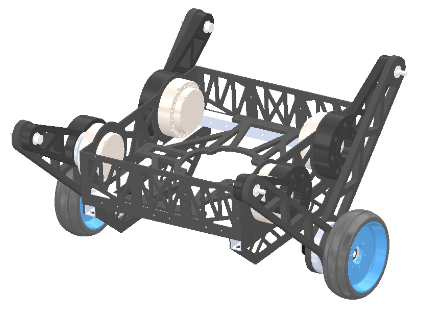
\includegraphics[scale=0.7]{../Mechanical Platform.png}
    \caption{\acrshort{wbr} Mechanical Platform}
    \label{fig:Mechanical Platform}
\end{figure}
This project is to develop the software and control system for a fully-autonomous delivery robot, based on the existing assembly of a \acrfull{wbr} provided by the \acrfull{macrm}, as shown in Figure \ref{fig:Mechanical Platform}. The project will be referred to as the \acrshort{wbr} project in the following documents.\\\\
For \acrshort{macrm}, \acrshort{wbr} was constructed following the constraints defined in the rules, \citet{RmuBuildSpecs2024}, of the 2024 \acrfull{rmul} Competition, whose host is \acrfull{dji}. Details of the constraints are shown in SRS \cite[see][Design Constraints]{SRS2023}. The hardware system is built under the competition constraints, that the robot shall be non-holonomic, able to balance itself on two wheels, and able to jump across obstacles. Here we are adapting it to our delivery robot project, and as the additional constraints for a delivery robot, it shall be able to plan and follow the delivery route, as well as automatically avoid obstacles on the way.

\subsection{Document Purpose}
The purpose of this document is to show the overall design of a system which meets the requirements stated in the SRS \cite[][]{SRS2023}. This includes the development team's decisions and considerations for system components, and also how we adapted the mechanical model (\acrshort{wbr}) built according to \acrfull{rmul} rules to our delivery robot project.

\subsection{Project Scope}
Since the mechanical and electronic hardware are fixed constraints, the \acrshort{wbr} project mainly focuses on the software and control system, while \acrshort{macrm} is responsible for the mechanical design, provision, and maintenance.

\subsection{Organization of Document}
The following document will outline the overall system components, communication protocols, overall system behavior, operation and undesired error handling.

\section{Project Overview}
\subsection{System Context}
\begin{figure}[H]
    \centering
    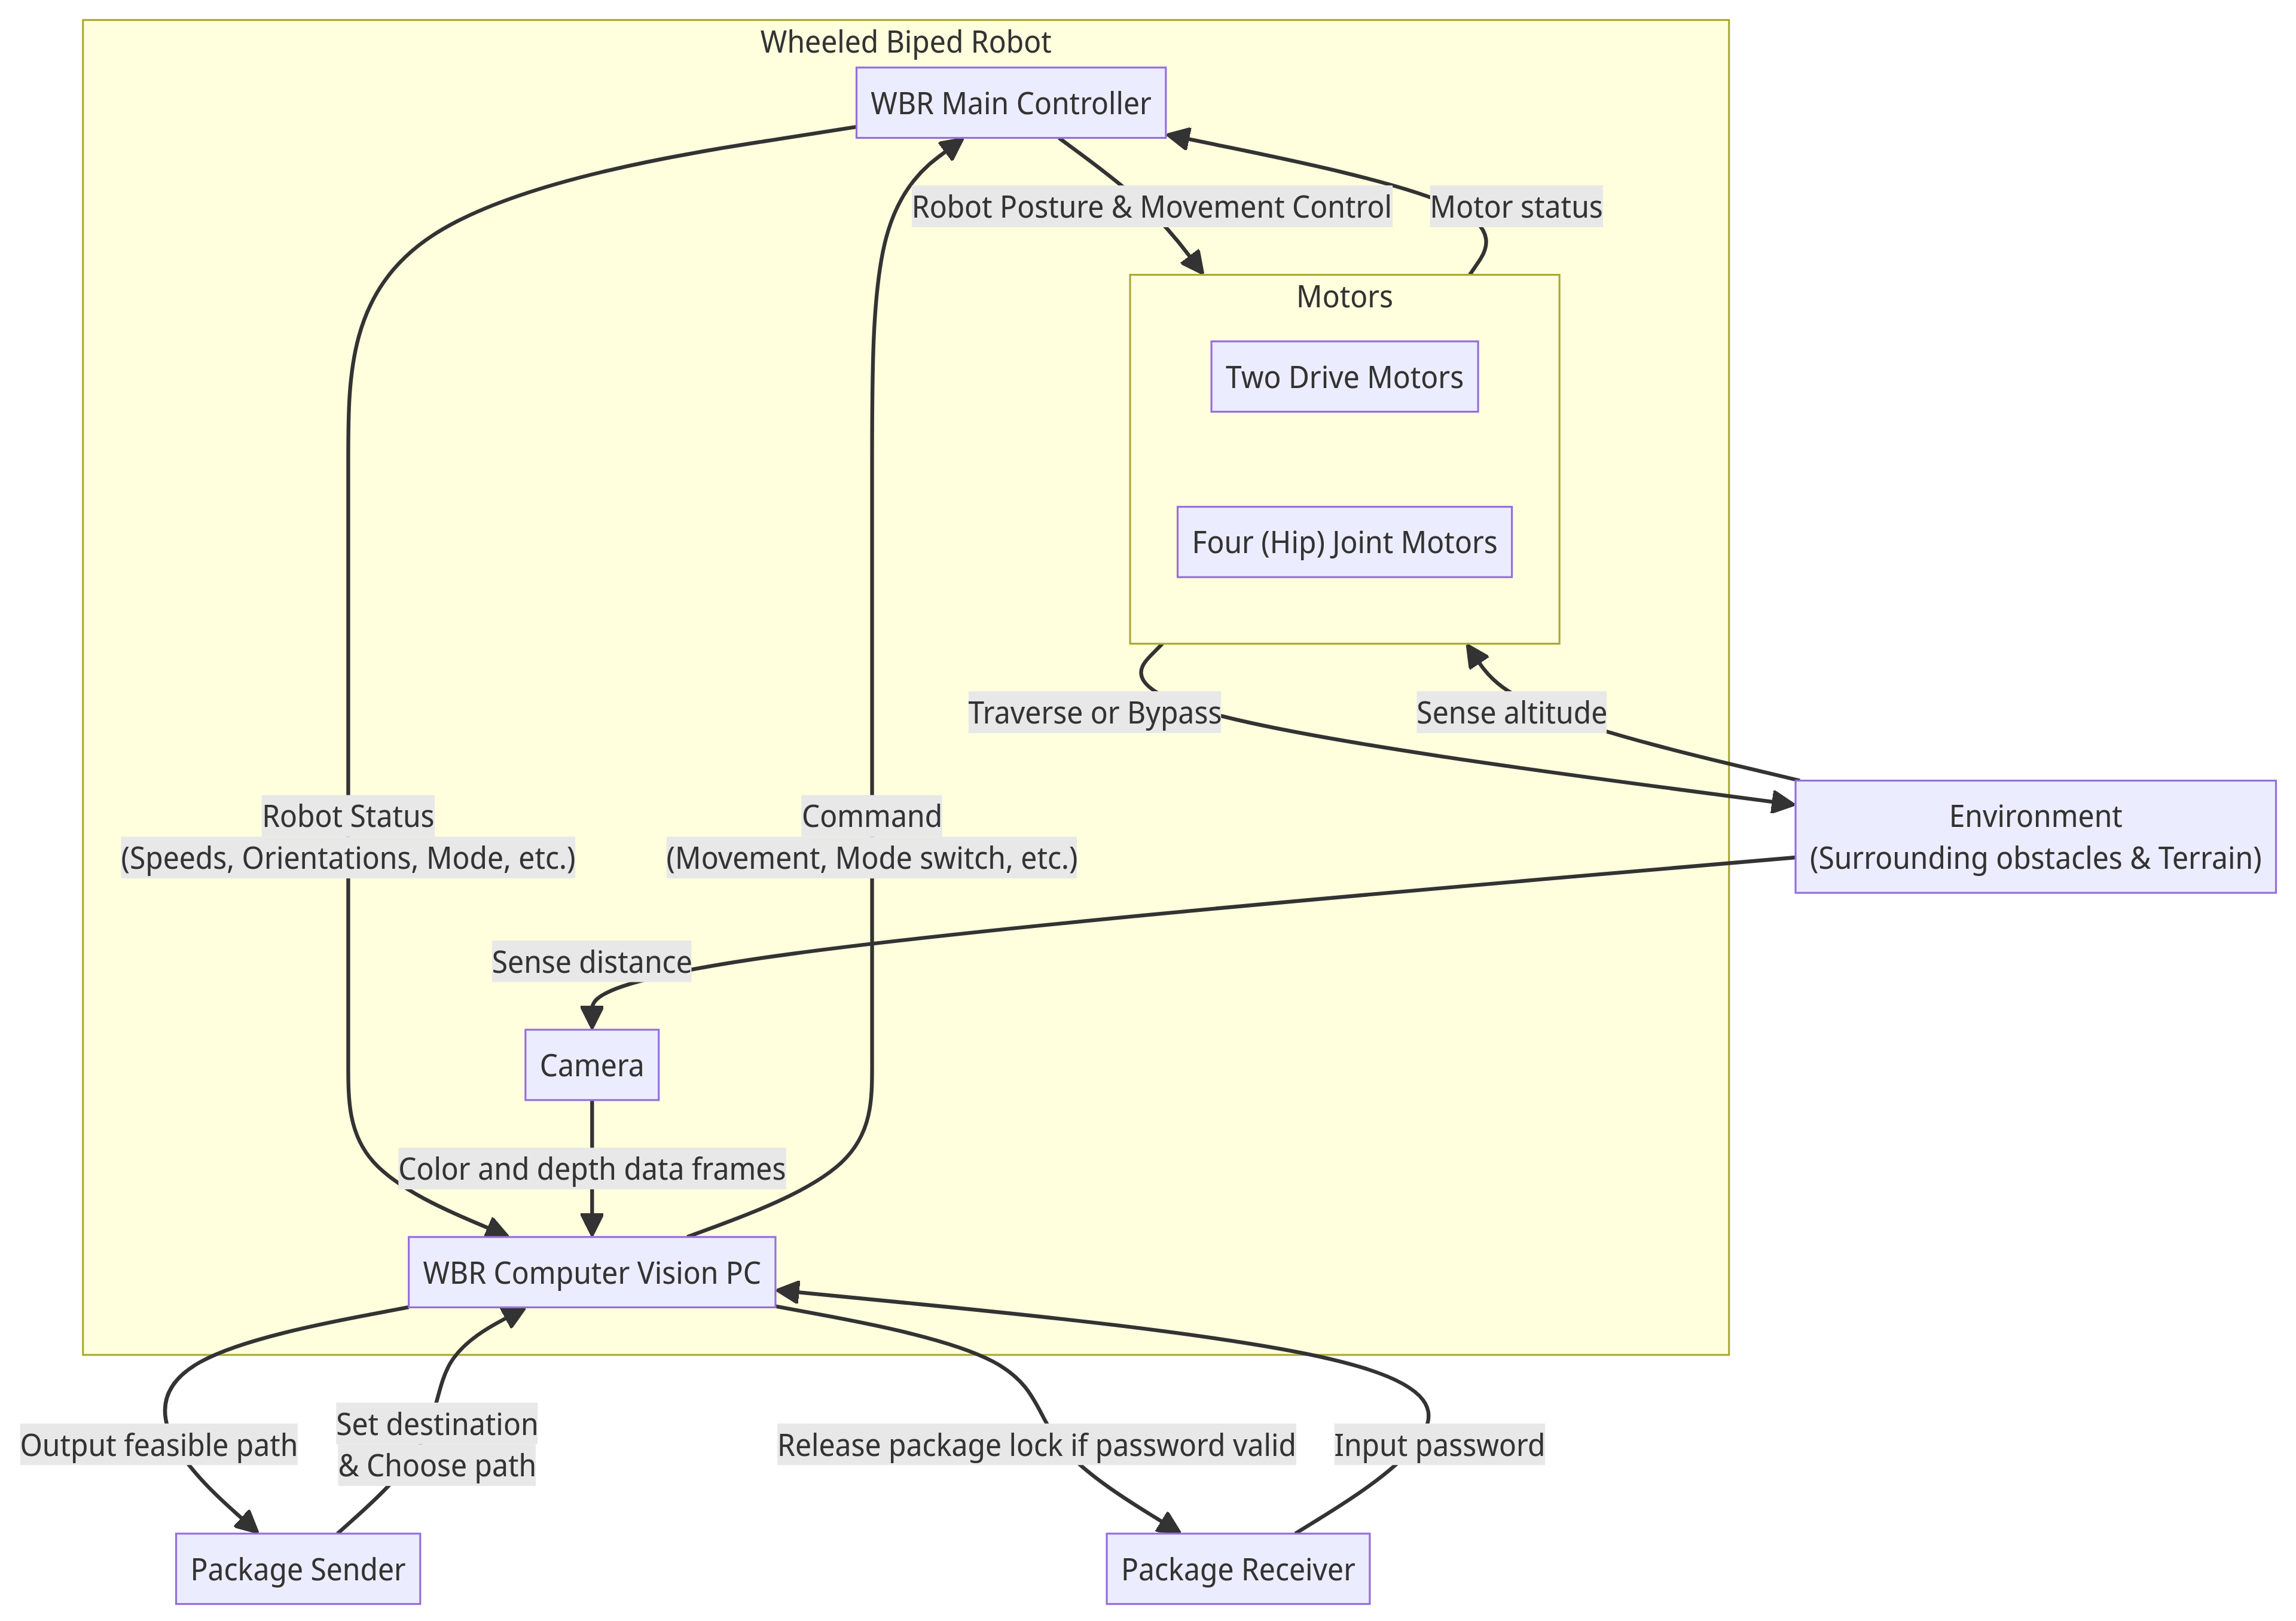
\includegraphics[width=\textwidth,height=\textheight,keepaspectratio]{../System Context Diagram.png}
    \caption{System Context Diagram}
\end{figure}
The following picture shows the design of the context diagram of the project, it illustrates the core interaction between the \acrshort{wbr} and its immediate external entities. In this diagram, the \acrshort{wbr} is the central system, the information regarding the condition of the environment is detected, such as the distance from the nearest obstacle, then the \acrshort{wbr} takes the reaction on how to handle a certain situation. The package sender acts as the external entity, it sets the destination and picks a route for the \acrshort{wbr} and the \acrshort{wbr} provides it the feasible path and goes to complete the package delivery. The package receiver is another external entitle, it inputs password, in response to it, the \acrshort{wbr} releases the package once it confirms the validity of the password.

\subsection{Hardware Platform}
    \subsubsection{Mechanical Platform}
    As mentioned in section \ref{sec:Project Purpose}, the \acrshort{wbr} is constrained by the rules of 2024 \acrshort{rmul}. From page 26 to 27 of the robot specification manual, \citet{RmuBuildSpecs2024}, our "Balancing Standard Robot" is constrained to have all ground-contacting surfaces aligned on the same line and cannot keep balance without dynamic adjustment. Additionally, to win the competition, the robot shall be light, fast, robust, and small.\\\\
    \begin{figure}[H]
        \centering
        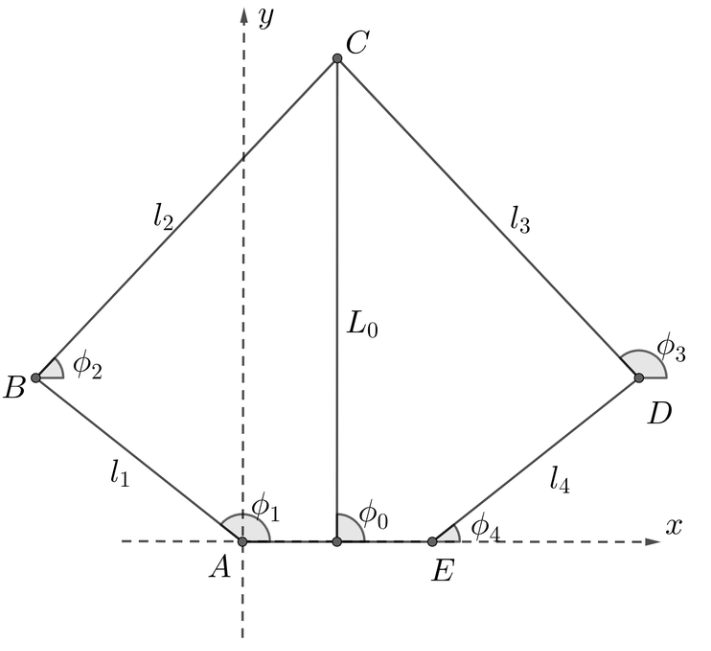
\includegraphics[scale=0.5]{../Leg Linkage.png}
        \caption{Sketch of \acrshort{wbr} Leg Linkage, from \citet{HarbinEngCtrlDesign2022}}
        \label{fig:Leg Linkage}
    \end{figure}
    Therefore, \acrshort{macrm} decided to put a five-bar linkage configuration on per side of the \acrshort{wbr}, by following the paper \citet{WbrBalanceControl2021}. Shape of each linkage, as illustrated in figure \ref{fig:Leg Linkage}, is controlled by a pair of two hip-joint motors, which changes the overall robot posture as a result. The two motors contacting the ground are drive motors, which regulates the horizontal movement.
    
    \subsubsection{Electronic Platform}
    \acrshort{macrm} designed the electronic system according to the rules of \acrshort{rmul} as shown in figure \ref{fig:WBR Electronic System}. The rationale of choice of each specific component is out of scope of this document.
    % \begin{figure}[H]
    \begin{sidewaysfigure}
        \centering
        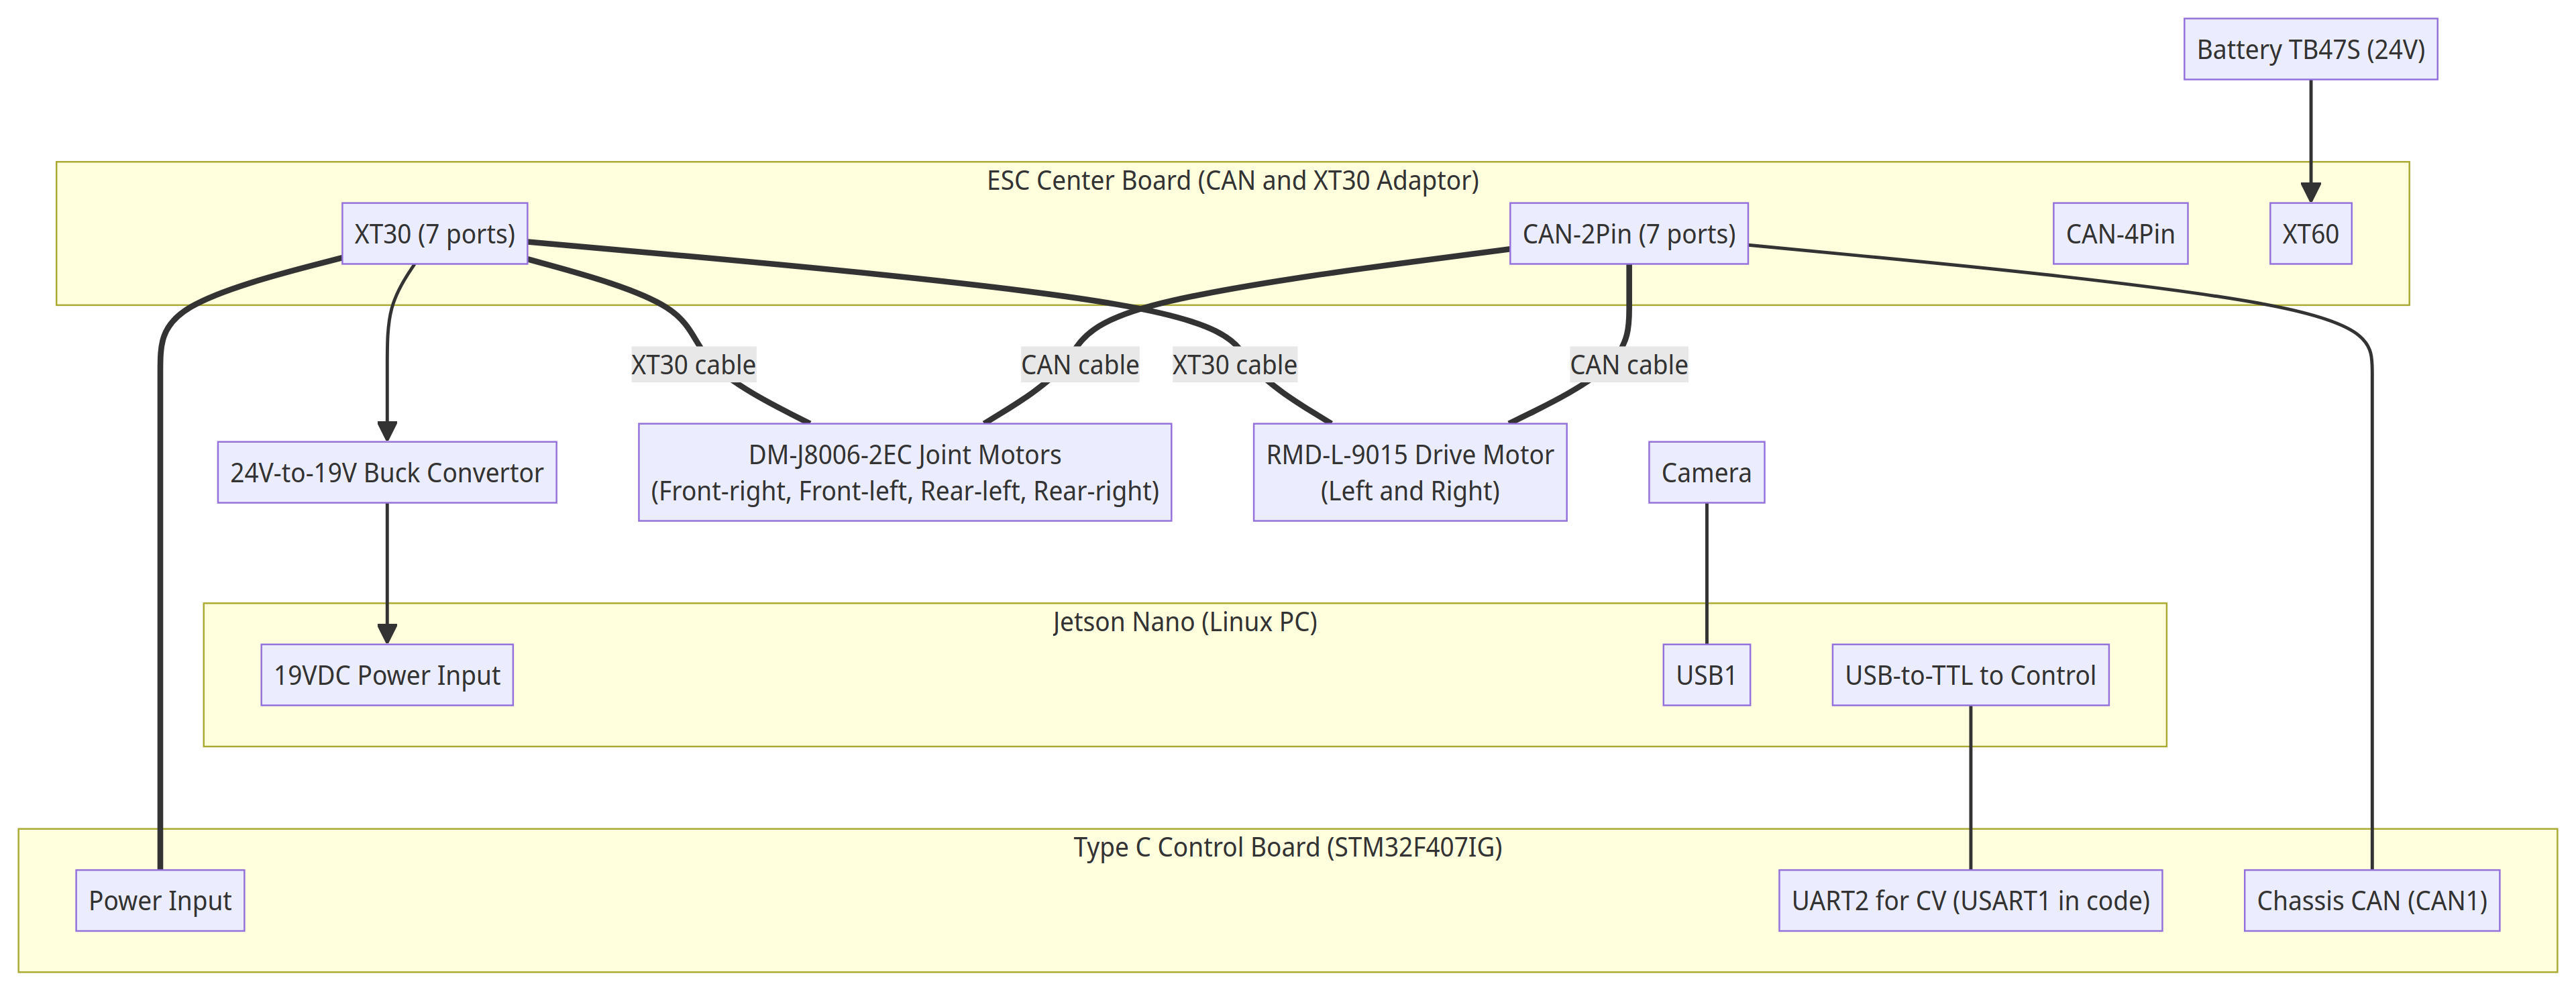
\includegraphics[width=\textwidth,height=\textheight,keepaspectratio]{../Electronic System Diagram.png}
        \caption{WBR Electronic System}
        \label{fig:WBR Electronic System}
    % \end{figure}
    \end{sidewaysfigure}
    % \end{landscape}

\section{System Variables} \label{sec:System Variables}    
    \subsection{Variables}
        \begin{table}[H]
            \caption{Monitored Variables}
            \begin{tabularx}{\textwidth}{|p{5cm}|p{2.5cm}|p{1.25cm}|X|}
                \toprule
                \textbf{Variable Name} & \textbf{Type} & \textbf{Unit}   & \textbf{Description}\\
                \midrule
                 m\_CameraReading & 2D list &  N/A & Output from last visual odometry reading compare to land.\\
                 m\_CurrentAcceleration & float & $m/s^2$  & Current Acceleration of WBR\\ 
                 m\_CurrentLocation & 2D list &  N/A  & The current location WBR is at.\\
                m\_CurrentRotation & 2D list & N/A & Current global Rotation in pitch yaw roll axis\\
                m\_CurrentSpeed  & float & $m/s$ & Current Speed of WBR\\
                m\_Destination & 2D list  & N/A & Final location that delivery need to go to.\\
                m\_GPSReading & 2D list &  N/A & Output from last GPS reading.\\
                m\_HipMotorAbsAngle & Digital Array & 0-max (TBD) & Encoder value of four hip motors\, measuring absolute angle.\\
                m\_IMUReading & 2D list &  N/A & Output from last IMU reading.\\
                m\_InitiaLocation & 2D list &  N/A  & m\_Initial Location that WBR is currently at\\
                m\_NextLocation & 2D list &  N/A & The next location WBR need to go to.\\
               m\_Orientation        & Analog Array  & \unit{\radian}  & Orientation of chassis\, to be sensed by \acrshort{imu}\\
               m\_TargetPitchAngle & Digital & m/s  & Commanded roll angle of chassis platform by CV.\\
               m\_TargetRollAngle & Digital & m/s & Commanded roll angle of chassis platform by CV.\\
               m\_Time                & Digital        & \unit{\second}  & Real-world time\\

                \bottomrule
            \end{tabularx}
        \end{table}

    
        \begin{table}[H]
            \caption{Controlled Variables}
            \begin{tabularx}{\textwidth}{|p{4cm}|p{2.5cm}|p{1cm}|X|}
                \toprule
                \textbf{Variable Name} & \textbf{Type} & \textbf{Unit} & \textbf{Description}           \\
                \midrule
                c\_CurrentLocation & 2D list &  N/A  & The current location WBR is at.\\
                c\_CurrentLocationVisual & 2D list &  N/A & Current global location of WBR.\\
                c\_DestinationArrived & Boolean &  N/A & Boolean to determine if destination is arrived or not.\\
                c\_DriveMotorTorques   & Digital Array & \unit{N.m}    & Desired torque of drive motors \\
                c\_EmailSent & Boolean &  N/A  & Boolean to determine if email is sent or not.\\
                c\_EstimatedLocation & 2D list &  N/A & Output from SLAM module that get estimation from sensor fusion.\\
                c\_GeoFence & 2D List & N/A & List and include all the point for geo boundaries.\\
                c\_HipMotorTorques  & Digital Array & \unit{N.m}    & Desired torque of hip motors   \\
                c\_ObstaclesLocations & 2D list &  N/A & Collection of local obstacles locations in list.\\
                c\_OnDelivery & Boolean &  N/A & Boolean to determine of delivery task is given or not.\\
                c\_ROSMap & 2D List & N/A  & Output that show all passable area.\\
                c\_TargetSpeed & float & $m/s$  & Target speed that it need to go to.\\
                c\_TrajectoryPath & 2D List & N/A & output that replace and insert into original path.\\
                \bottomrule
            \end{tabularx}
        \end{table}
    
        \begin{table}[H]
            \caption{Enumerated Variables}
            \begin{tabularx}{\textwidth}{|p{3cm}|X|X|}
                \toprule
                \textbf{Enumerated Name} & \textbf{Description} & \textbf{Range}                         \\
                \midrule
                y\_Posture               & Robot posture state  & \{e\_Jump, e\_Normal, \acrshort{tbd}\} \\
                y\_TargetPosture              & Commanded target posture state of robot  & \{e\_Jump, e\_Normal, \acrshort{tbd}\} \\
                
                
                \bottomrule
            \end{tabularx}
        \end{table}
    
    \subsection{Constants}
        Almost all constants are not yet determined, but will be after details of mechanical model is finalized, assembled, and measured by \acrshort{macrm}.
        \begin{table}[H]
            \caption{Constants}
            \begin{tabularx}{\textwidth}{|p{6cm}|p{1.5cm}|p{1.25cm}|p{1cm}|X|}
                \toprule
                \textbf{Constant Name} & \textbf{Type} & \textbf{Unit} & \textbf{Value} & \textbf{Description} \\
                \midrule
                k\_JumpTimeout         & Digital       & \si{second} & TBD & The maximum amount of time the \acrshort{wbr} shall finish any stage of jump mode                     \\
                k\_PidGains            & Digital Array & \acrshort{na} &TBD & Gains for each \acrshort{pid} controller feedbacks.                                                   \\
                k\_L1Length            & Digital       & \si{m}      & TBD & Length of link l1 in figure \ref{fig:Leg Linkage}. Note that linkages on left and right sides are symmetric. \\
                k\_L2Length            & Digital       & \si{m}    &  TBD  & Length of link l2 in figure \ref{fig:Leg Linkage}. Note that linkages on left and right sides are symmetric. \\
                k\_L3Length            & Digital       & \si{m}    &  TBD  & Length of link l3 in figure \ref{fig:Leg Linkage}. Note that linkages on left and right sides are symmetric. \\
                k\_L4Length            & Digital       & \si{m}     & TBD  & Length of link l4 in figure \ref{fig:Leg Linkage}. Note that linkages on left and right sides are symmetric. \\
                k\_MaxEquivLegLength              & Digital       & \si{m}    & TBD   & The maximum allowable equivalent length WBR can reach                                         \\
                k\_MinEquivLegLength              & Digital       & \si{m}    & TBD   & The minimum allowable equivalent length WBR can reach                                          \\
                k\_MaxEquivLegLength              & Digital       & \si{m}    & TBD   & The maximum allowable equivalent length WBR can reach                                         \\
                k\_PidGains            & Digital Array & \acrshort{na} &TBD & Gains for each \acrshort{pid} controller feedbacks.                                                   \\
                k\_RawMap & 3D List &  N/A  &TBD & Input image being read as RGB 3D List.\\
                k\_RobotMass           & Digital       & \si{kg}    & TBD  & Approximate mass of robot without cargo.                                                              \\
                k\_WindowSize & float & m & TBD& Windows size that we need to update path with\\

                \bottomrule
            \end{tabularx}
        \end{table}
        
\section{System Behaviour Overview}
    \subsection{Normal Operation}
        To make the behaviour of the product to achieve the target task, the Finite State Machine is created to describe the behaviour with detailed description provided after the picture.
        \begin{figure}[H]
            \centering
            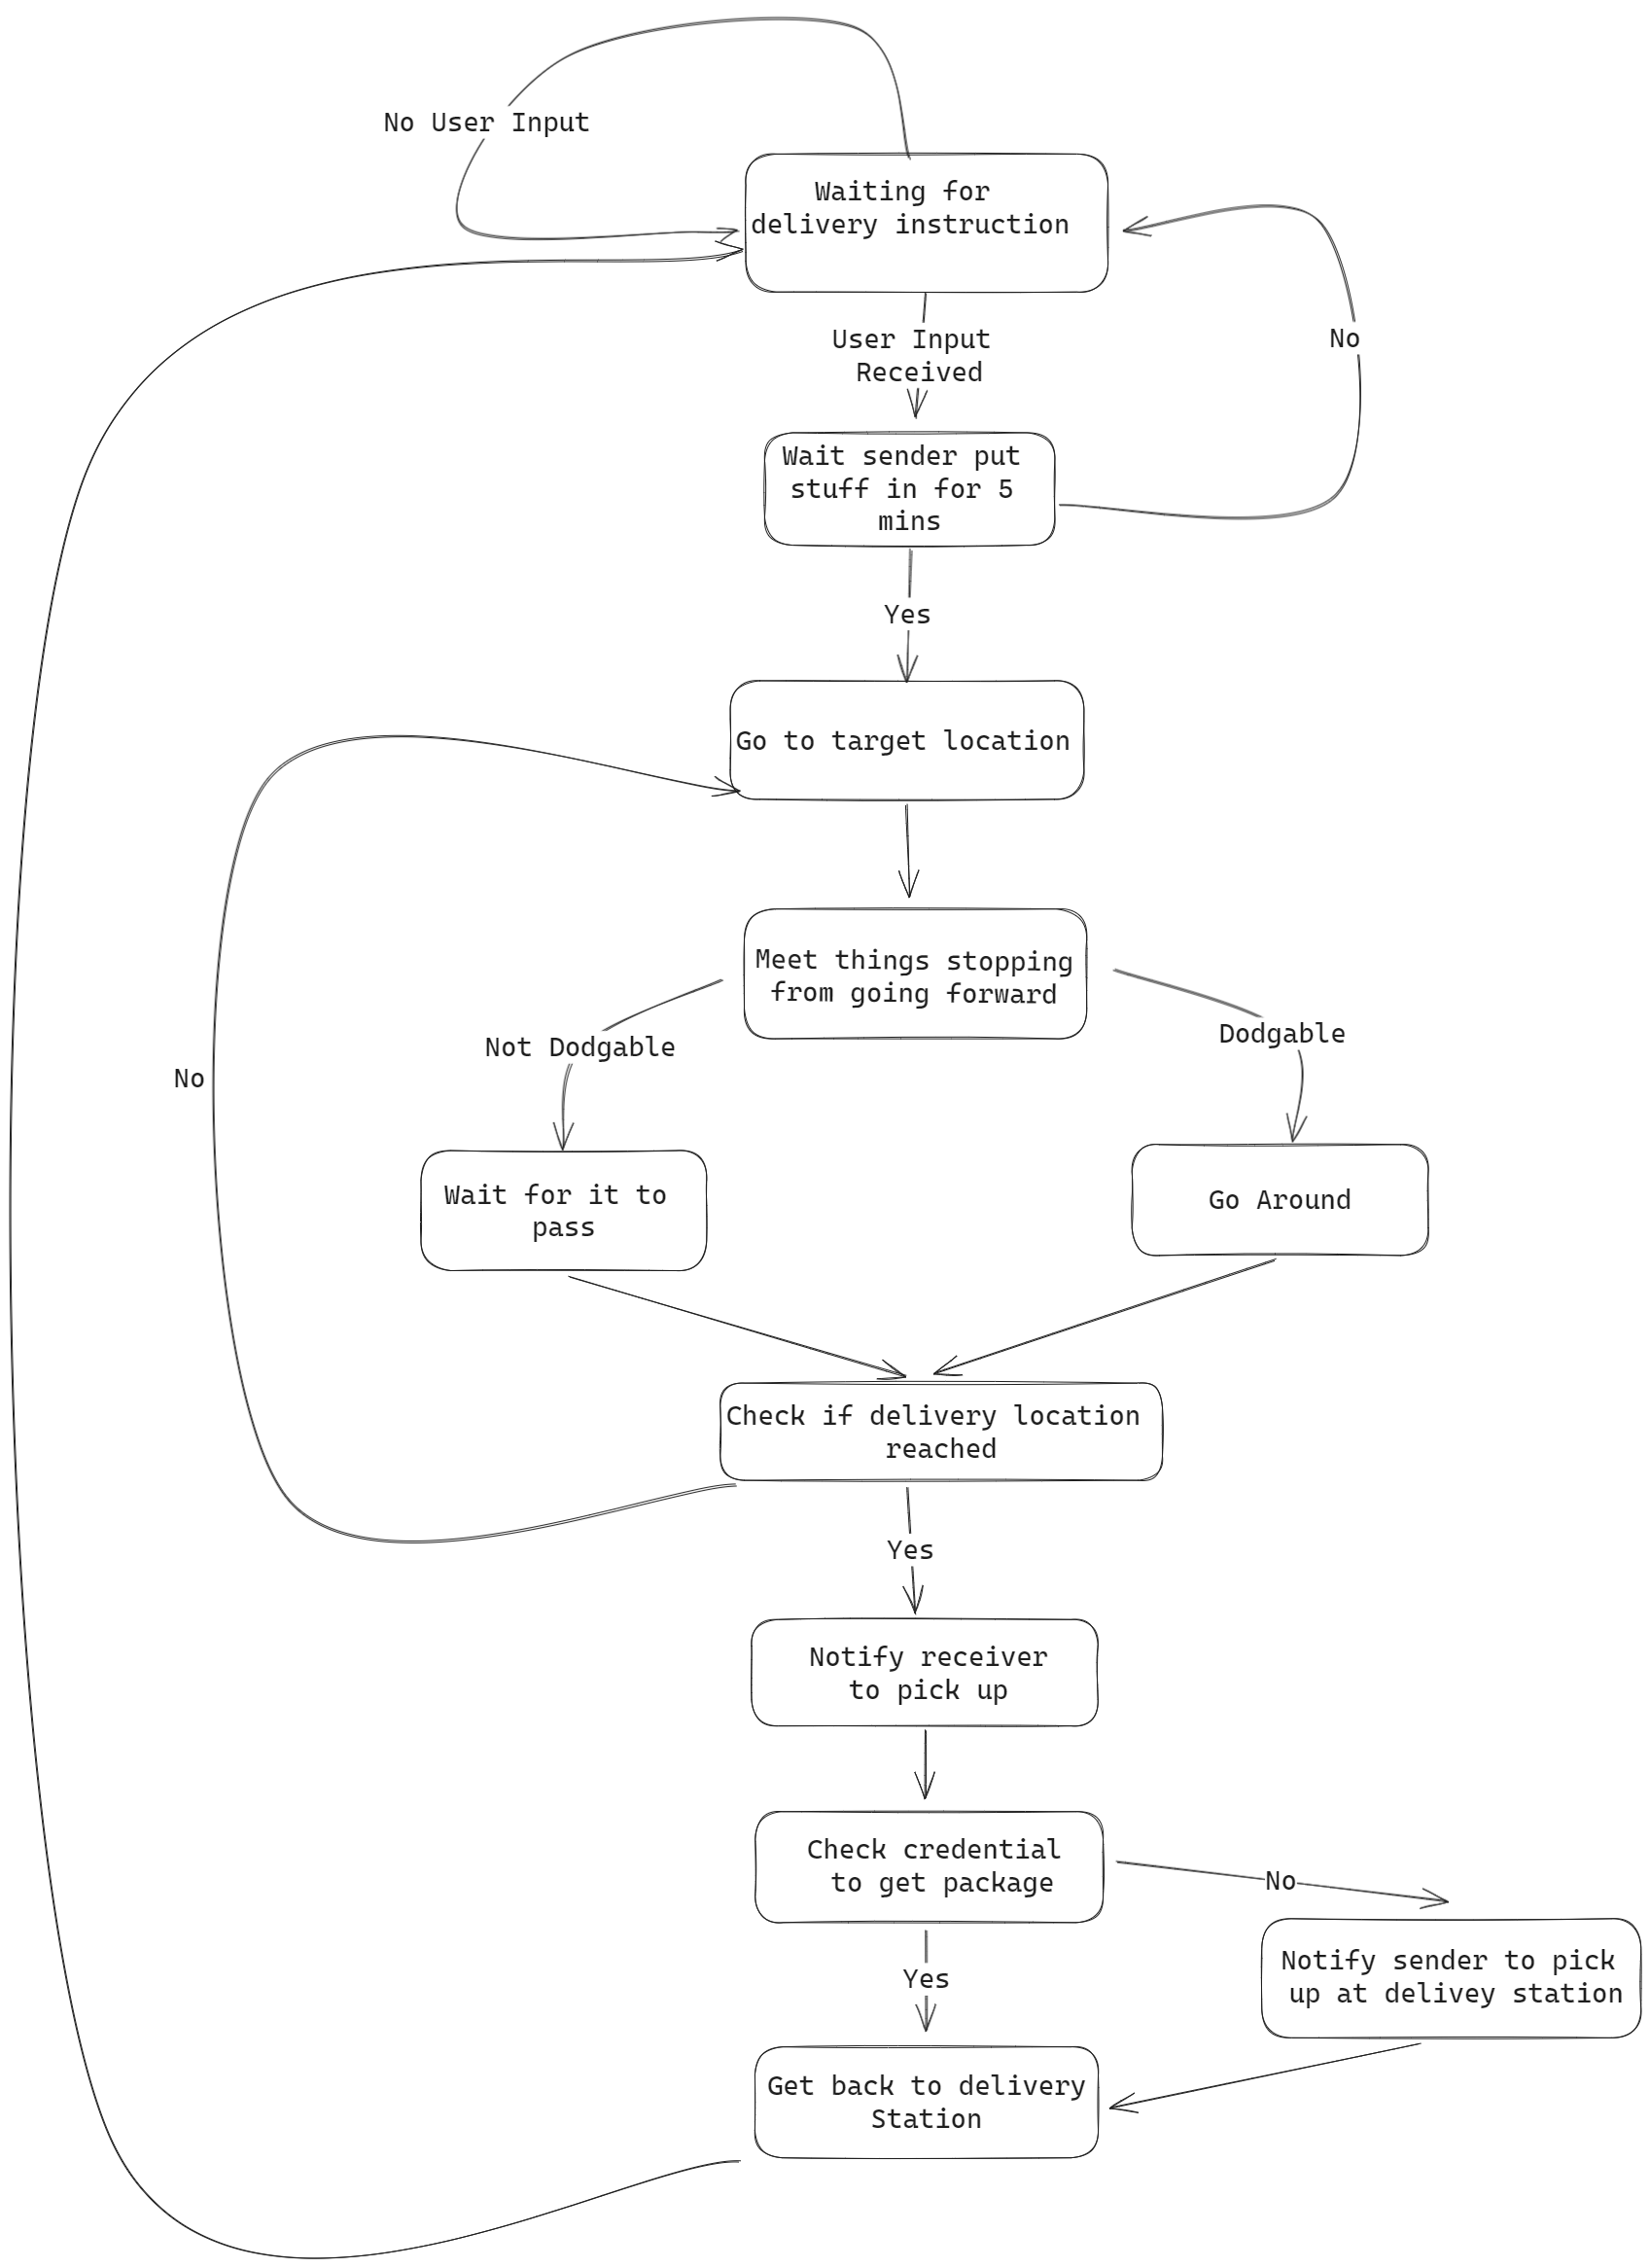
\includegraphics[width=\textwidth,height=\textheight,keepaspectratio]{../state-machine.png}
            \caption{System Behaviour in Finite State Machine}
        \end{figure}
    
    \subsection{Normal Operation State Descriptions}    
        The Finite State Machine diagram briefly introduces the following general behaviours state. The description is given below:\\\\
        \noindent\textbf{Waiting for delivery instruction:} It will need to stay in the delivery station to wait for new delivery instructions coming in from a client \\\\
        \noindent\textbf{Wait sender put stuff in for 5 mins:} Upon receiving a  delivery instruction, the robot initiates waiting status to allow sender side client to put stuff in delivery box for 5 mins. If there is nothing inside after 5 mins, it will return back the first status to waiting next delivery instruction\\\\
        \textbf{Go to target location:} After sender side client put stuff in for delivery. Robot will start navigation to the target location. \\\\
        \textbf{Meet things stopping from going forward :} When the sensor detects nearby obstacles, it communicates this information to the control system. The system temporarily interrupts the ongoing path travel task and initiates the execution of a special task.\\\\
        \textbf{Check if delivery location reached:} When going closer to the delivery location or algorithm detect \acrshort{wbr} reached target destination. It will go check if it actually reached or not.\\\\
        \textbf{Notify Reciver to pick up :} After comfirming the target destination is reached, \acrshort{wbr} will notify Reciver to pick package up. \\\\
        \textbf{Check credential to get package :} This status will ensure only the person will credential can get the package, other wise it will bring the package back to original delivery station.  \\\\
        \textbf{Get back to delivery Station :} After finishing delivery task, it will go back to delivery station for next delivery task or wait there until previous failed delivery to be pick up. \\\\
    
    \subsection{Undesired Event Handling}
        The robot's undesired event handling is designed to ensure a high level of safety and operational integrity in various challenging scenarios. In the case of a collision or obstacle blocking, the robot promptly initiates an emergency stop to prevent any potential harm, followed by attempts to re-plan its path to navigate around the obstacle, prioritizing safety and adaptability. Loss of communication triggers the robot to make efforts to re-establish the link; if unsuccessful within a predefined time, it enters a safe mode, ceasing movements and alerting operators to prevent uncontrolled actions. In the event of a system fault, the robot logs the error, performs self-diagnosis, and initiates an emergency stop if necessary, providing detailed reports for maintenance teams to ensure quick troubleshooting and repairs. Human interference is addressed by the robot's safe response, avoiding collisions, initiating emergency stops when required, and alerting operators to prioritize human safety. Loss of localization prompts the robot to re-establish its position; if unsuccessful, it enters a safe mode to prevent unpredictable behavior in the absence of accurate localization. These well-defined responses demonstrate a comprehensive approach to handling undesired events, emphasizing safety, adaptability, and effective communication with operators and maintenance teams.\\\\
          Managing unexpected situations or errors during the operation of the Wheeled Biped Robot (WBP) is essential. Therefore, it is crucial to be aware of all potential events and to compile a comprehensive list summarizing these unexpected occurrences. All the possible unexpected events are listed below:
          \begin{itemize}
          \item \textbf{Collision or Obstacle Blocking:} occurs when the robot encounters physical obstacles or collides with objects and potentially impeding its movements, which potentially terminates its operation.
          \item  \textbf{Loss of Communication:} Involves disruption between the robot and external environment.
          \item  \textbf{System Fault:} This includes the malfunction or the failure of internal components or the error in software programs. 
          \item  \textbf{Human Interface:} Issues between robot and the human operators.
          \item  \textbf{Loss of Localization:} This occurs when the robot losses its sense of position or orientation.

          \end{itemize}        

\section{System Components}
    Below is a chart showing how the modules were decomposed. The following subsections act as the individual module guide.
    \begin{figure}[H]
        \centering
        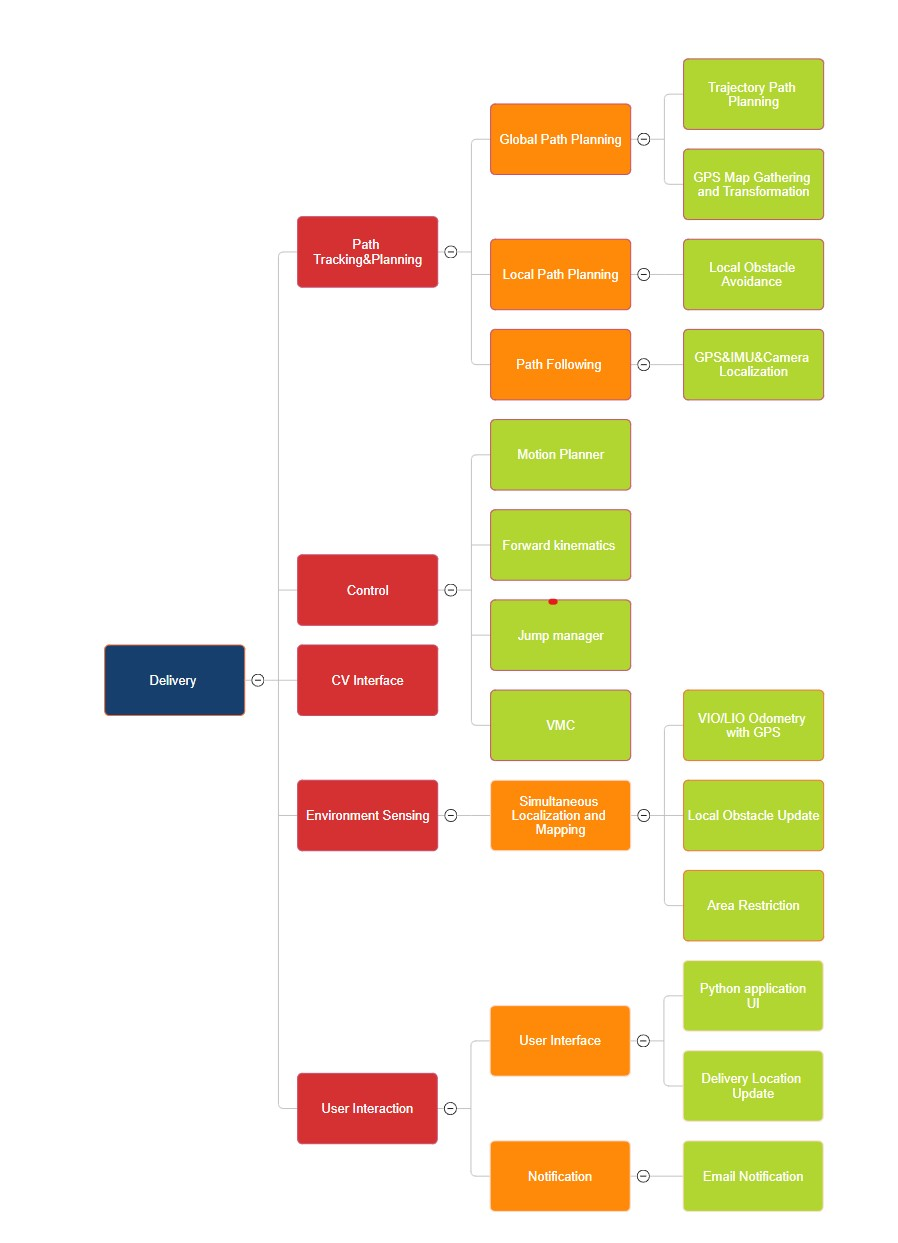
\includegraphics[width=\textwidth,height=\textheight,keepaspectratio]{../Decomp_Tree.jpg}
        \caption{Modular Decomposition Tree}
    \end{figure}
    
    \begin{figure}[H]
        \centering
        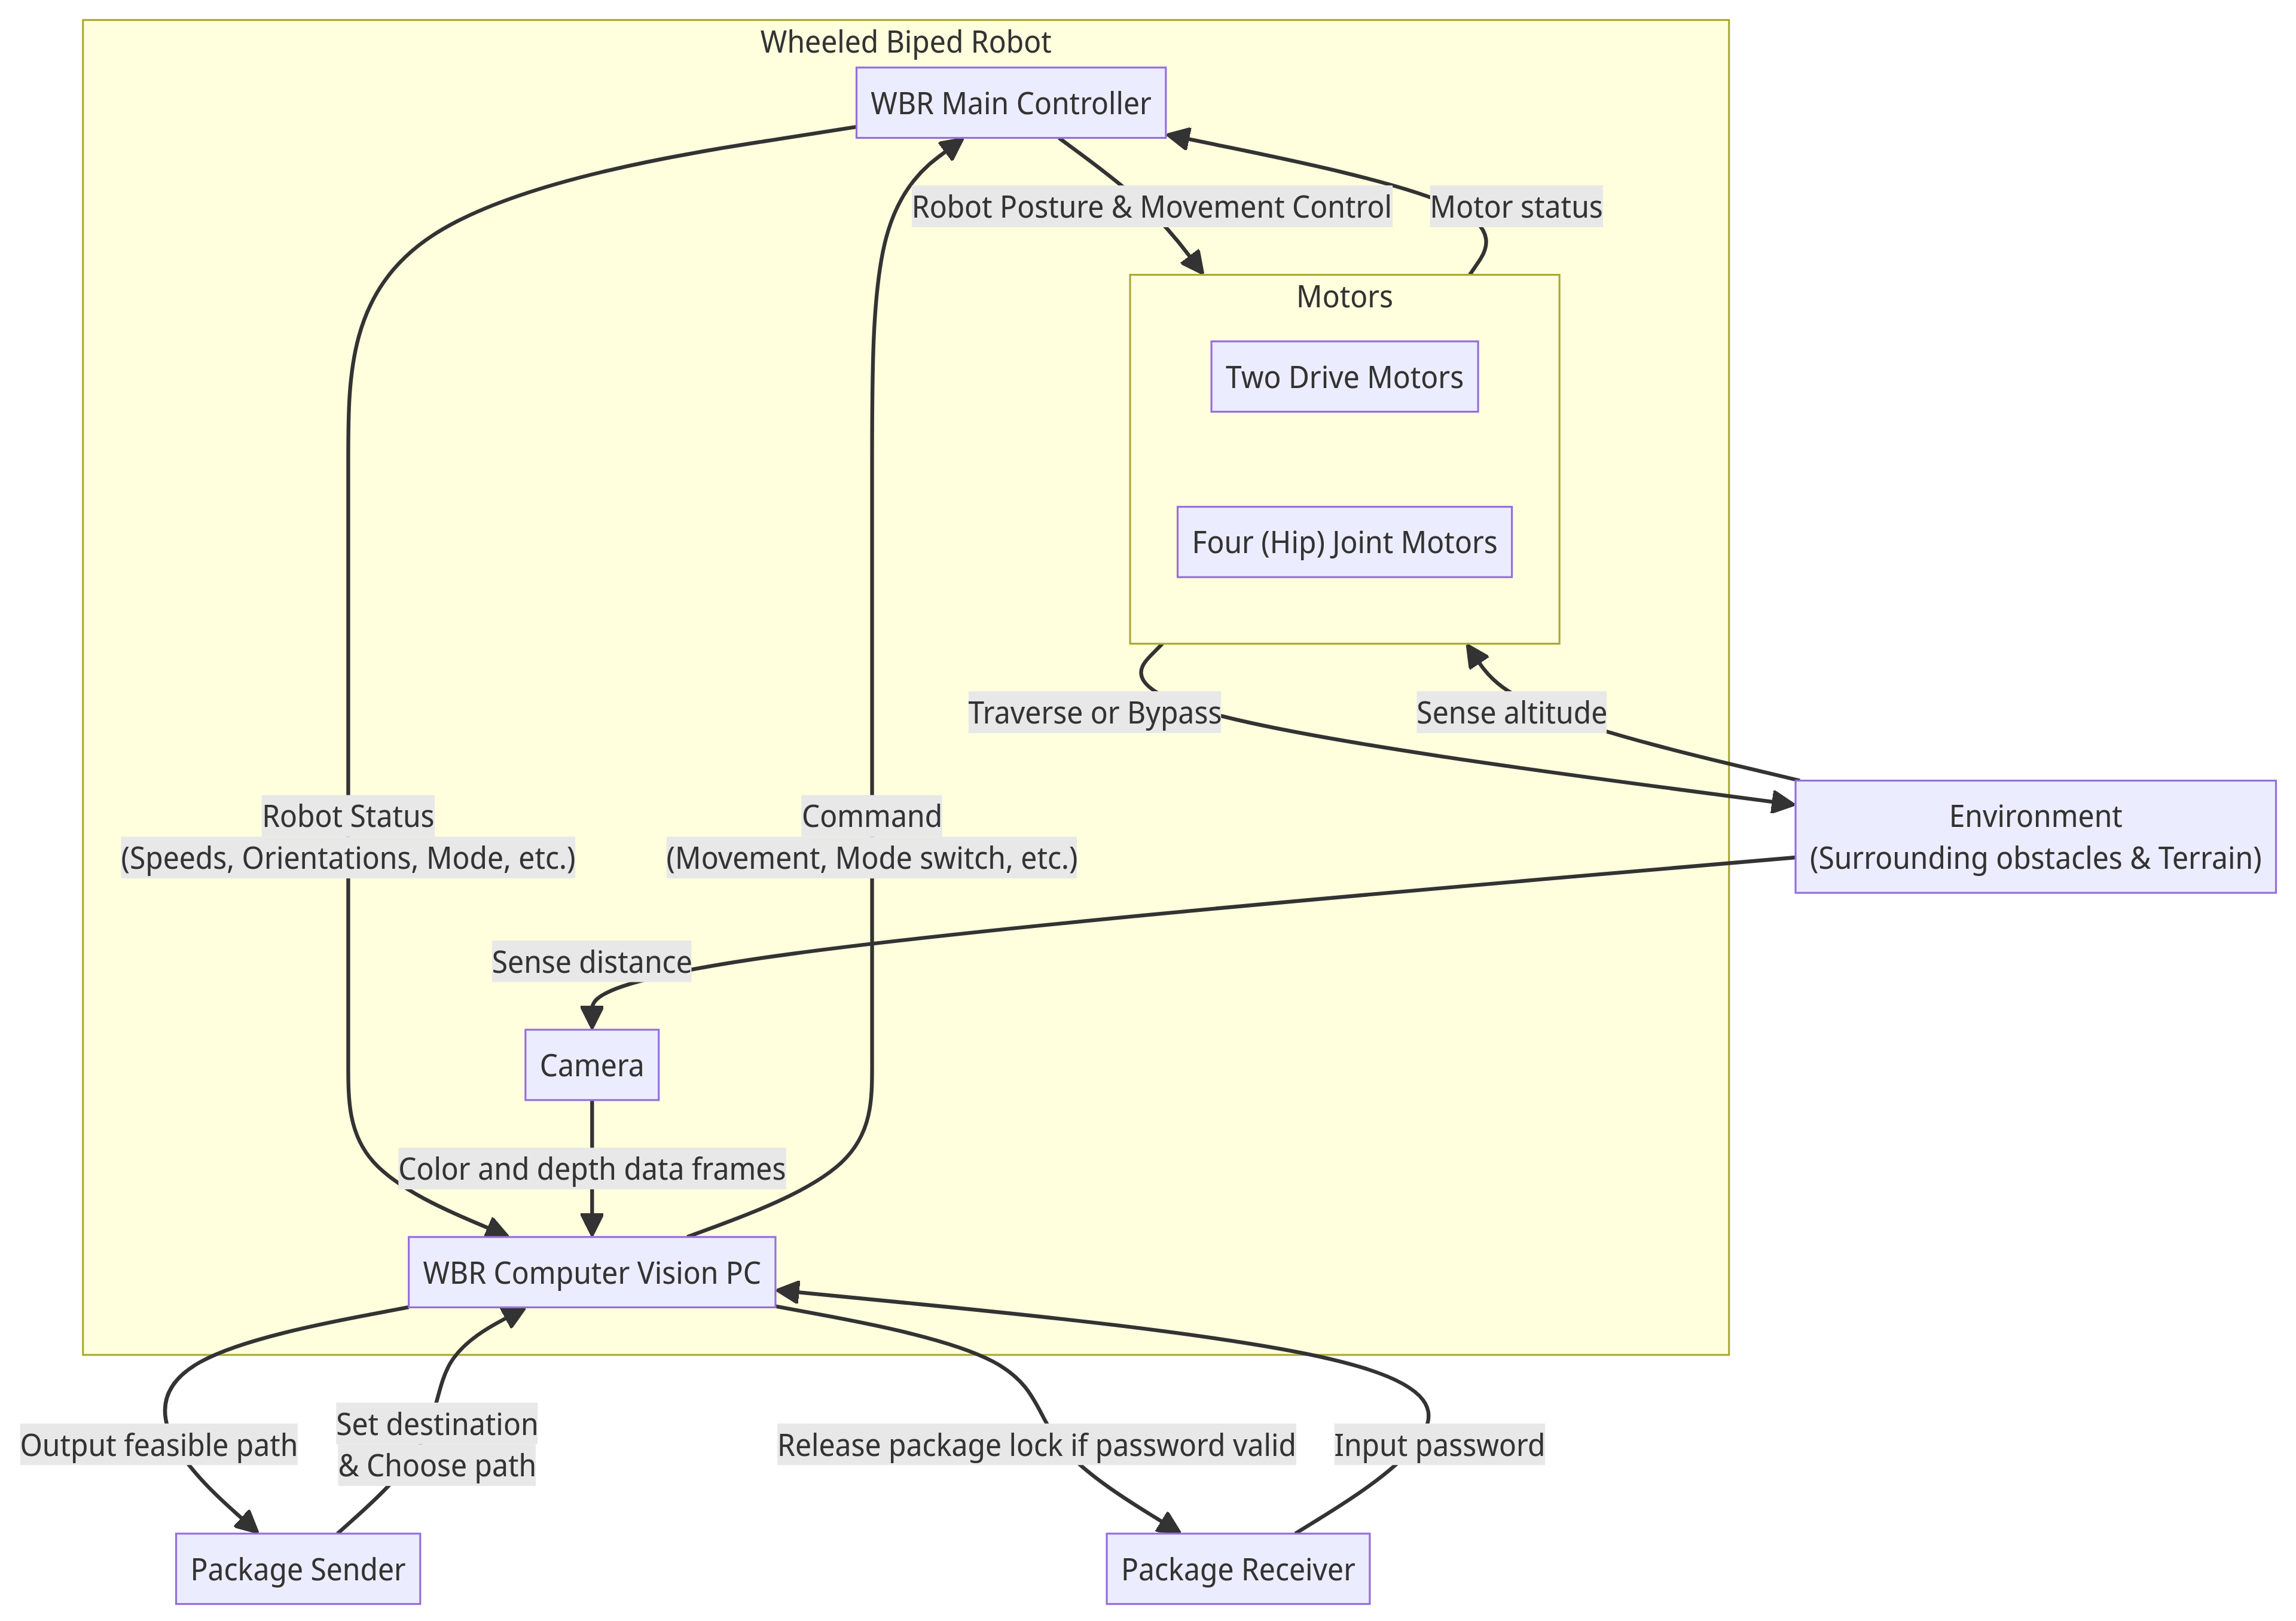
\includegraphics[width=\textwidth,height=\textheight,keepaspectratio]{../Complete System Diagram.png}
        \caption{Complete System Diagram}
    \end{figure}
    \newpage
    \subsection{Path Tracking \& Planning Module}
        \subsubsection{Global Path Planning: Trajectory Path Planning}
            \begin{figure}[H]
                \centering
                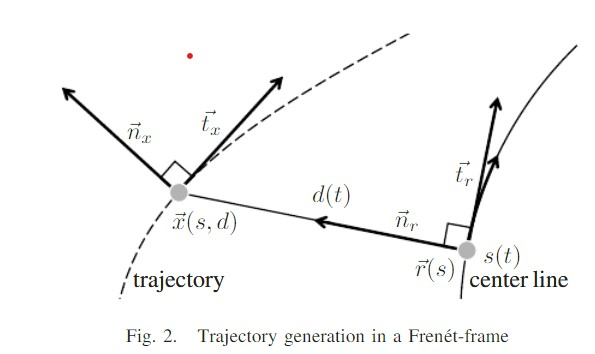
\includegraphics{../Trajectory.jpg}
                \caption{Optimal Trajectory Path Generation}
            \end{figure} 
            \paragraph{Description} 
                ~\newline
                This module is the sub module for global path planning module. In order to get better path and less error during path tracking period, we need to choose trajectory path planning for WBR, \cite{inproceedings}. \\\\
                Using this algorithm we should able to get smooth movement on WBR.
                And the following expressions describe our trajectory path generation. x(s(t),d(t)) is the result Trajectory Path.
                \[
                    \vec{x}(s(t),d(t))=\vec{r}(s(t))+d(t)\vec{n_r}(s(t))
                \]
                
            \paragraph{Inputs}
                ~\newline
                \begin{table}[H]
                  \centering
                    \caption{Input Variables of Trajectory Path Planning Module} \label{tbl:Input Variables of Trajectory Path Planning Module}
                  \begin{tabularx}{\textwidth}{|p{5cm}|p{2cm}|p{1.2cm}|p{1cm}|X|}
                    \hline Variable Name & Variable Type & Units & Range & Description \\
                    \hline m\_InitiaLocation & 2D list &  N/A & TBD & m\_Initial Location that WBR is currently at\\
                    \hline m\_CurrentSpeed  & float & m/s & TBD & Current Speed of WBR\\
                    \hline m\_CurrentAcceleration & float & $m/s^2$ & TBD & Current Acceleration of WBR\\
                    \hline m\_Destination & 2D list  & N/A & TBD & Final location that delivery need to go to.\\
                    \hline
                  \end{tabularx}
                \end{table}
            
            \paragraph{Outputs}
                ~\newline
                \begin{table}[H]
                  \centering
                    \caption{Output Variables of Trajectory Path Planning Module} \label{tbl:Output Variables of Trajectory Path Planning Module}
                  \begin{tabularx}{\textwidth}{|p{5cm}|p{1.2cm}|p{1.2cm}|p{1cm}|X|}
                    \hline Variable Name & Variable Type & Units & Range & Description \\
                    \hline c\_TrajectoryPath & 2D list &  N/A & TBD & Collection of points that WBR need follow alone the way.\\
                    \hline
                  \end{tabularx}
                \end{table}
                
            \paragraph{Exception Handling}
                ~\newline
                If destination is not in the range of area restriction (Geo Fence Area) system will give out warning to sender on python interface with. Then ask for re-enter the destination. \\
                Any illegal input will give out warning and refuse to continue to next step.    
            \paragraph{Timing Constraints}
                ~\newline
                This module will finish within 2 mins of input being given. 
            \paragraph{Initialization}
                ~\newline
                Reset all to zero.
        \newpage
        
        \subsubsection{Global Path Planning : GPS Map Gathering and Transformation}
            \paragraph{Description}
                \begin{figure}[H]
                    \centering
                    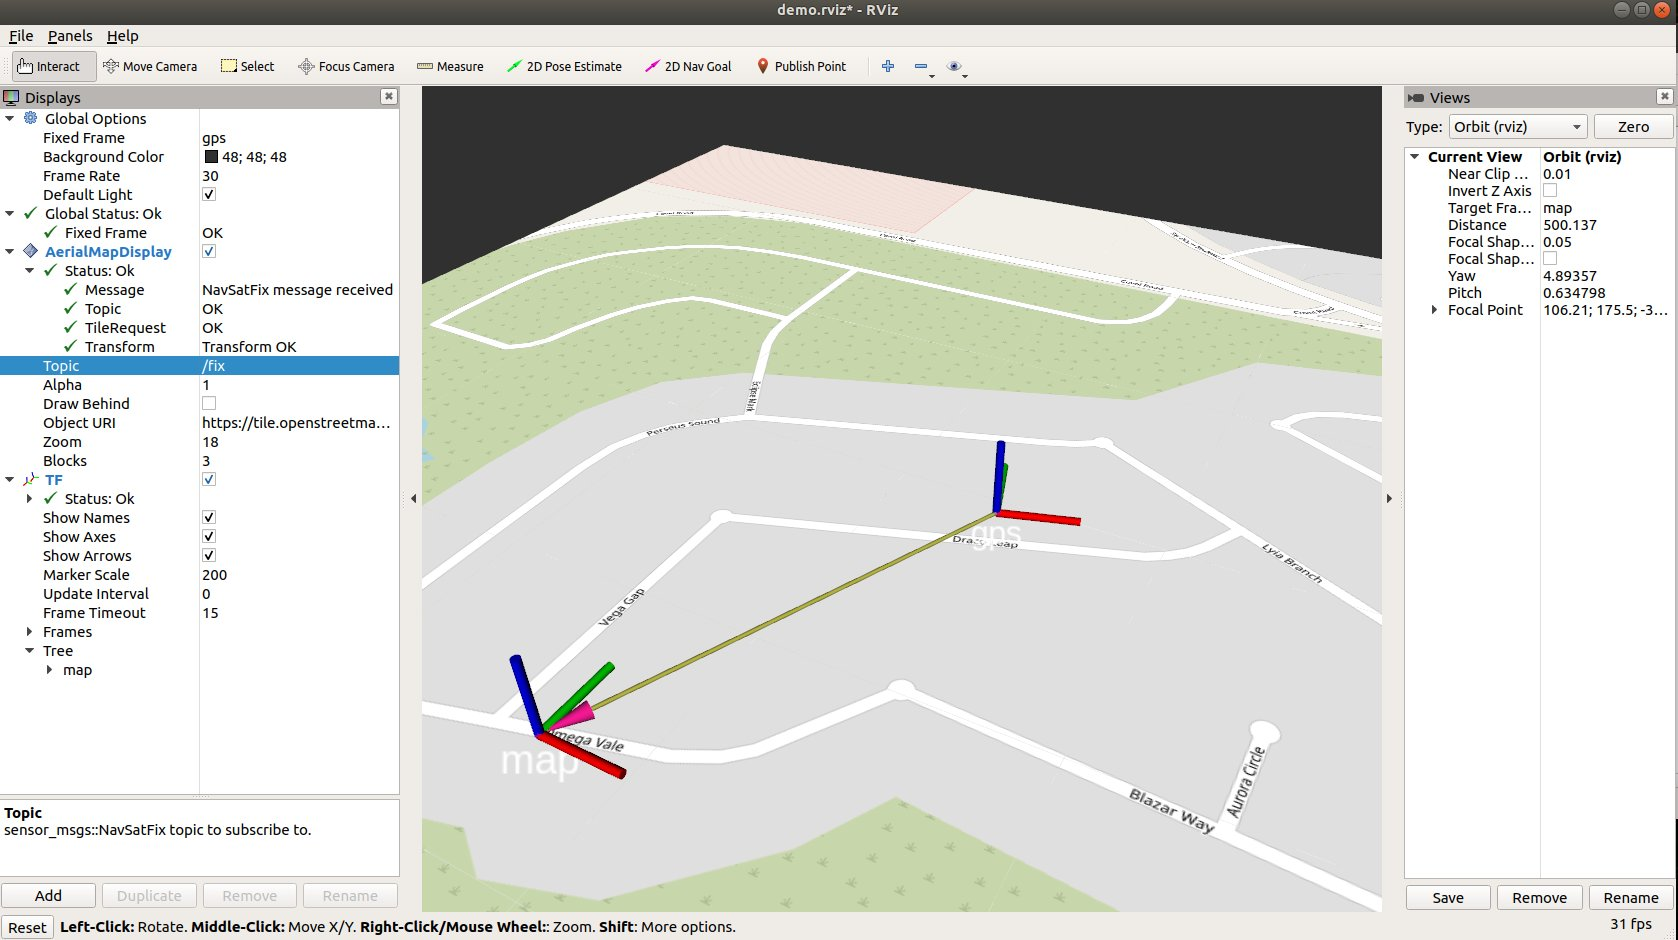
\includegraphics[width=\textwidth,height=\textheight,keepaspectratio]{../localization.png}
                    \caption{Map Gathering and Transformation}
                \end{figure}
                ~\newline
                This module is to transfer google map to grid map or other style of map that system can read for localization. We need to extra the image from google map to gather are that we want WBR to work within. Then output a grid map or other map format that can be used for localization with enough accuracy.  \\
                This module will be ran before put WBR into work. Since This is in the initialization process for the entire system. 
            \paragraph{Inputs}
                ~\newline
                \begin{table}[H]
                  \centering
                    \caption{Input Variables of GPS Map Gathering and Transformation} \label{tbl:Input Variables of GPS Map Gathering and Transformation}
                  \begin{tabularx}{\textwidth}{|p{5cm}|p{2cm}|p{1.2cm}|p{1cm}|X|}
                    \hline Variable Name & Variable Type & Units & Range & Description \\
                    \hline k\_RawMap & 3D List &  N/A & TBD & Input image being read as RGB 3D List.\\
                    \hline
                  \end{tabularx}
                \end{table}            
                
            \paragraph{Outputs}
                ~\newline
                \begin{table}[H]
                  \centering
                    \caption{Output Variables of GPS Map Gathering and Transformation} 
                    \label{tbl:Output Variables of GPS Map Gathering and Transformation}
                  \begin{tabularx}{\textwidth}{|p{5cm}|p{2cm}|p{1.2cm}|p{1cm}|X|}
                    \hline Variable Name & Variable Type & Units & Range & Description \\
                    \hline c\_ROSMap & 2D List & N/A & TBD & Output that show all passable area.\\
                    \hline
                  \end{tabularx}
                \end{table} 
                
            \paragraph{Exception Handling}
                ~\newline
                We will do a manual double check on the grid map generation to make sure there are no bad boundaries on the generated map. \\
                At the same time, during WBR working condition, there will also be a Geo Fence applied to it on GPS that connect to internet in real-time. 
                
            \paragraph{Timing Constraints}
                ~\newline
                Since this module need to be ran ahead of everything. The time constrain is very little, as long as it is able to finish in 10 mins, we will accept the time.
                
            \paragraph{Initialization}
                ~\newline
                Reset the output variable to zero and make sure there are enough storage for both map and image.
                
        \subsubsection{Local Path Planning : Local Obstacle Avoidance}
            \paragraph{Description}
                \begin{figure}[H]
                    \centering
                    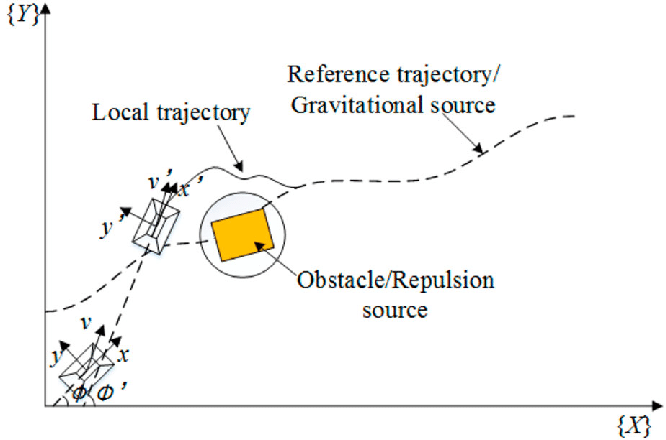
\includegraphics[width=\textwidth,height=\textheight,keepaspectratio]{../local_obstacle.png}
                    \caption{Local Obstacle Avoidance}
                \end{figure}
                ~\newline
                Local obstacle avoidance is a critical component in creating safe and reliable autonomous systems that can navigate complex and dynamic environments. Its successful implementation contributes to the overall efficiency and safety of robotic and autonomous applications in various fields. During delivery task, there are many unexpected obstacle that will show up, for example person, car, bike, cart, and animals. We need to make sure that all obstacle that are not on the original grid map will be dodged. 
                The idea is gathered from \cite{article} paper" Active vehicle obstacle avoidance based on integrated horizontal and vertical control strategy".
                Since this is an local obstacle avoidance for path planning, we will make a window within the size of environment sensing area and it need to react ahead of time. \\
                
            \paragraph{Inputs}
                ~\newline
                \begin{table}[H]
                  \centering
                    \caption{Input Variables of Local Obstacle Avoidance} \label{tbl:Input Variables of Local Obstacle Avoidance}
                  \begin{tabularx}{\textwidth}{|p{5cm}|p{2cm}|p{1.2cm}|p{1cm}|X|}
                    \hline Variable Name & Variable Type & Units & Range & Description \\
                    \hline c\_TrajectoryPath & 2D list &  N/A & TBD & Collection of points that WBR need follow alone the way.\\
                    \hline c\_ObstaclesLocations & 2D list &  N/A & TBD & Collection of local obstacles locations in list.\\
                    \hline m\_CurrentSpeed  & float & $m/s$ & TBD & Current Speed of WBR\\
                    \hline m\_CurrentAcceleration & float & $m/s^2$ & TBD & Current Acceleration of WBR\\
                    \hline k\_WindowSize & float & m & TBD & Windows size that we need to update path with\\
                    \hline
                  \end{tabularx}
                \end{table} 
                
            \paragraph{Outputs}
                ~\newline
                \begin{table}[H]
                  \centering
                    \caption{Output Variables of Local Obstacle Avoidance} 
                    \label{tbl:Output Variables of Local Obstacle Avoidance}
                  \begin{tabularx}{\textwidth}{|p{5cm}|p{2cm}|p{1.2cm}|p{1cm}|X|}
                    \hline Variable Name & Variable Type & Units & Range & Description \\
                    \hline c\_TrajectoryPath & 2D List & N/A & TBD & output that replace and insert into original path.\\
                    \hline
                  \end{tabularx}
                \end{table} 
                
            \paragraph{Exception Handling}
                ~\newline
                If SLAM update information slower than expected, the windows size will be increase at the same time. And If obstacle can not be avoid with Current Speed and acceleration, we will performance emergency stop. 
                                
            \paragraph{Timing Constraints}
                ~\newline
                This module need to finish in 100ms which is 10 Hz frequency that same as the frequency of LiDAR/Camera. 
                
            \paragraph{Initialization}       
                ~\newline
                Gather information from system and set windows size according to 10 Hz frequency.
                
        \subsubsection{Path Following : GPS,IMU, and Camera Localization}
            \begin{figure}[H]
                \centering
                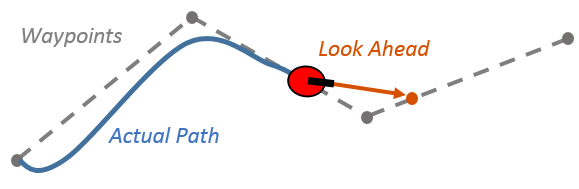
\includegraphics[width=\textwidth,height=\textheight,keepaspectratio]{../path_following.png}
                \caption{Path Following Concept}
            \end{figure}
            
            \paragraph{Description}        
                ~\newline
                This module runs with input from SLAM module that sensor fusion for GPS, IMU, and LIO/VIO have been applied. We take the final estimated location for the robot and plan the next movement based on current location. 
                \begin{figure}[H]
                    \centering
                    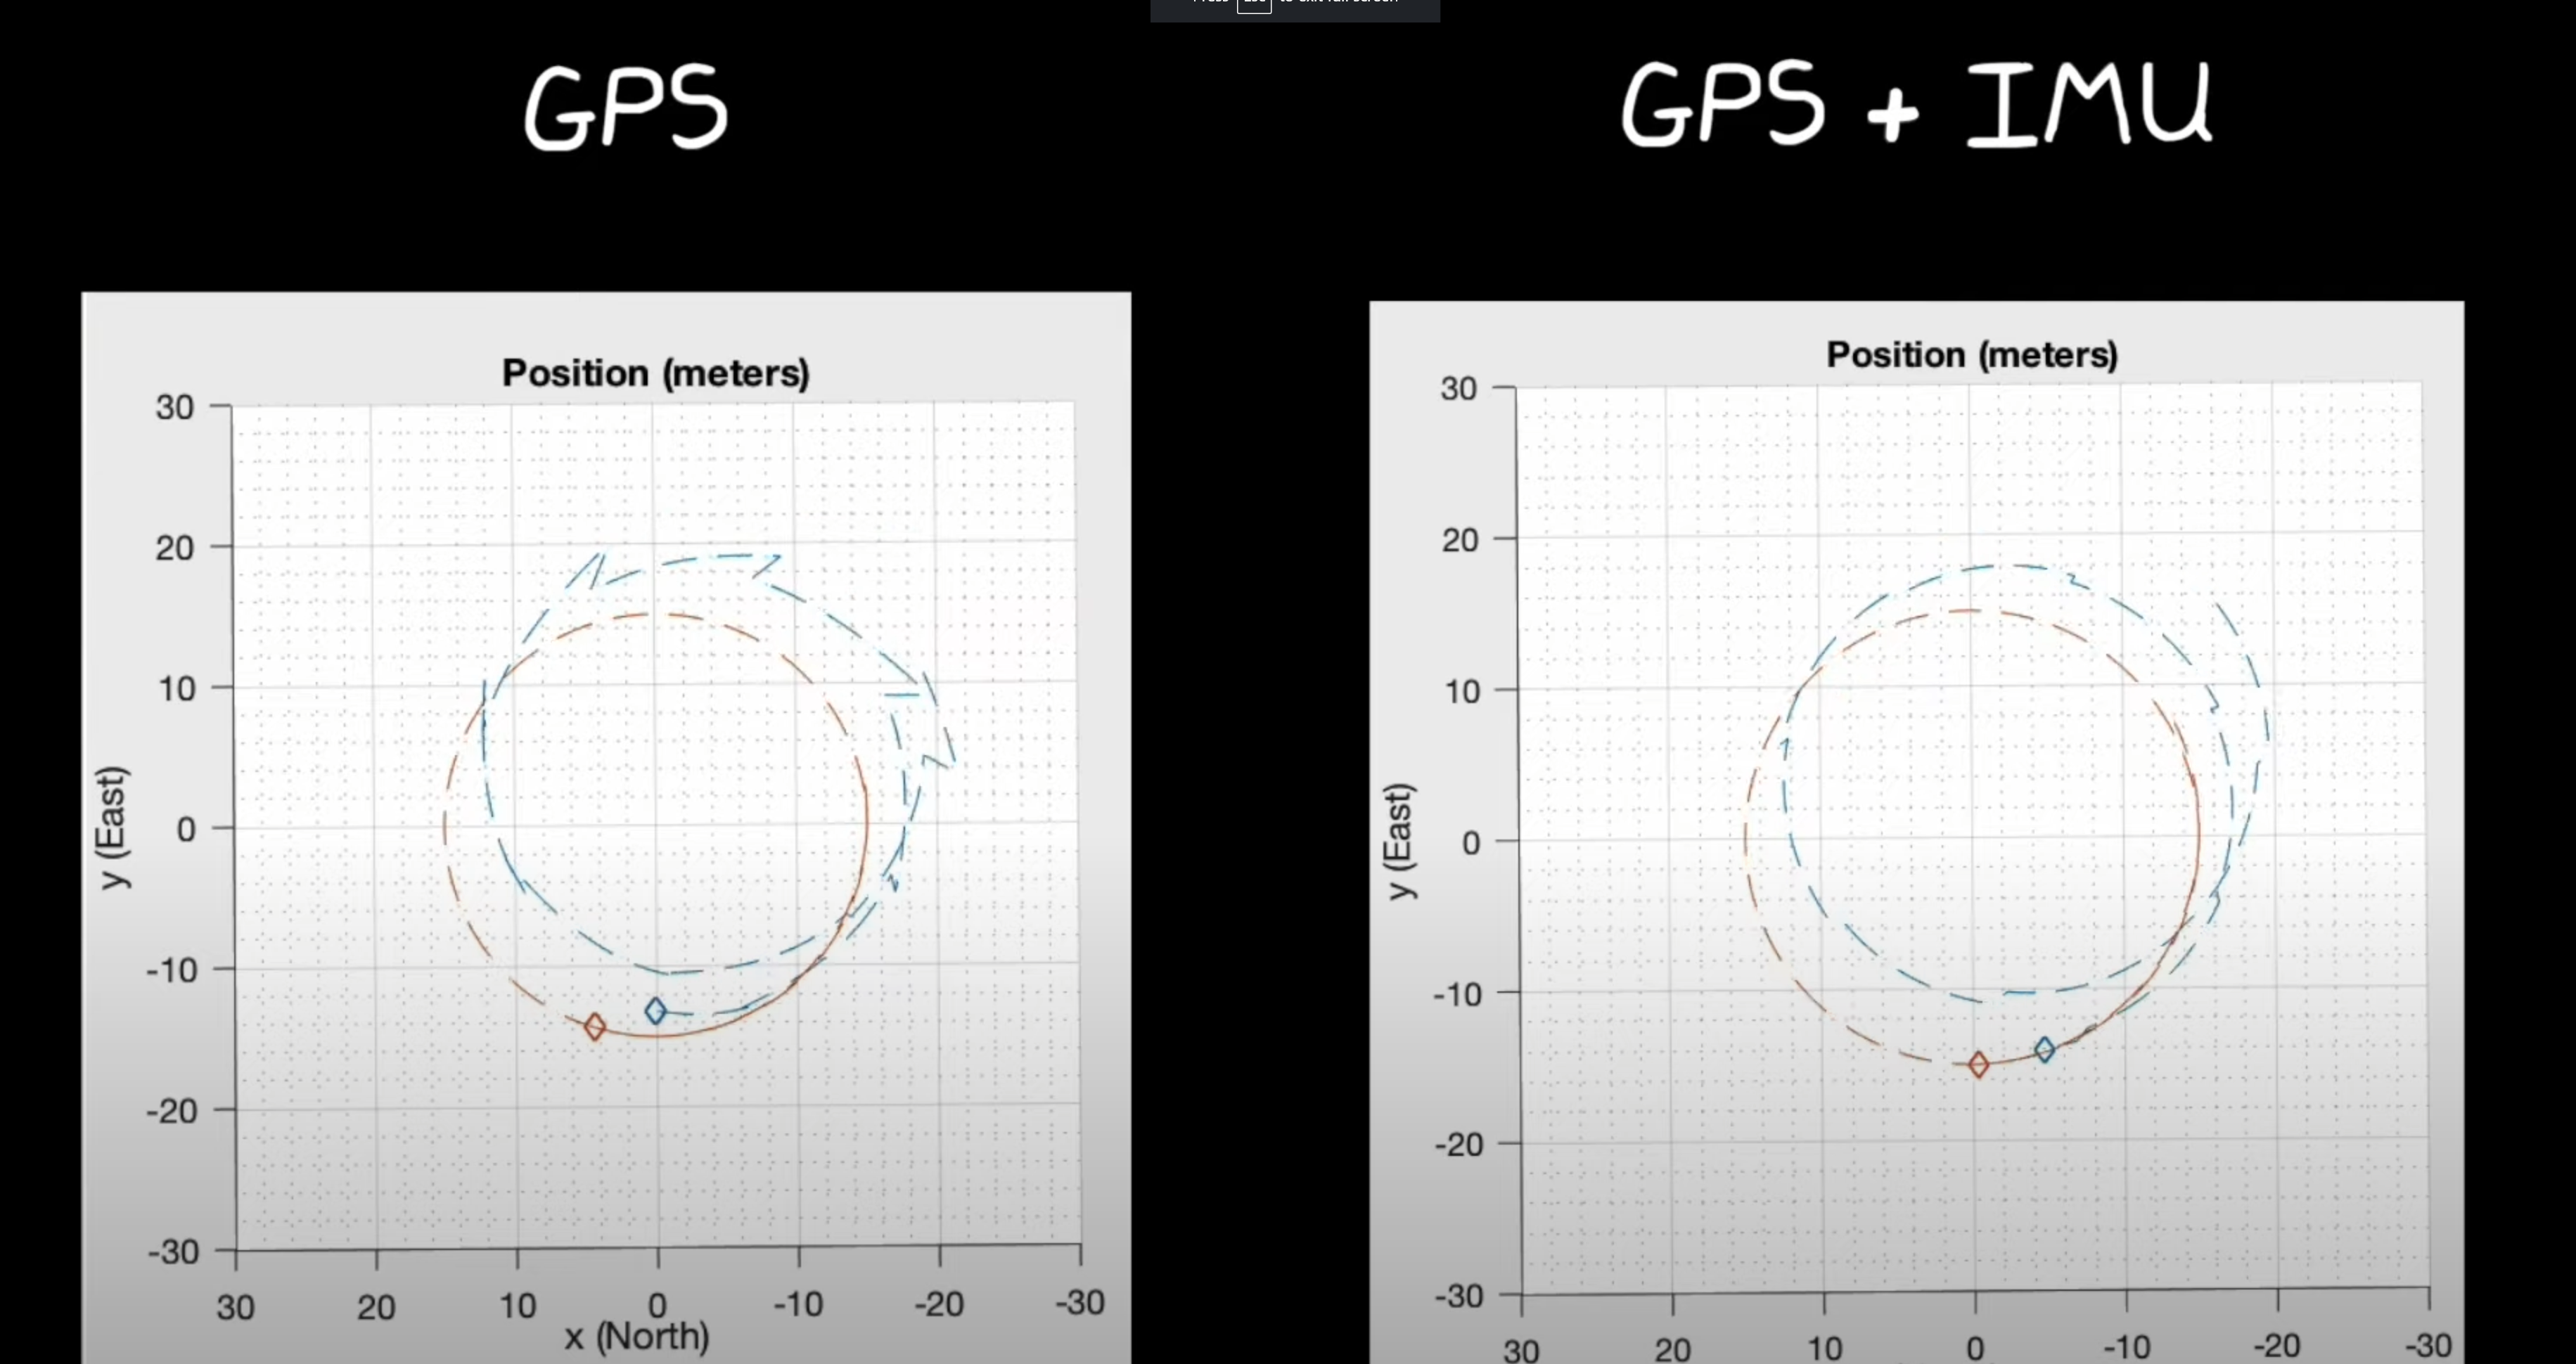
\includegraphics[width=\textwidth,height=\textheight,keepaspectratio]{../sensor_fusion.png}
                    \caption{Sensor Fusion Result Comparison}
                \end{figure}
                
            \paragraph{Inputs}
                ~\newline
                \begin{table}[H]
                  \centering
                    \caption{Input Variables of GPS,IMU, and Camera Localization} \label{tbl:Input Variables of GPS,IMU, and Camera Localization}
                  \begin{tabularx}{\textwidth}{|p{5cm}|p{2cm}|p{1.2cm}|p{1cm}|X|}
                    \hline Variable Name & Variable Type & Units & Range & Description \\
                    \hline c\_EstimatedLocation & 2D list &  N/A & TBD & Output from SLAM module that get estimation from sensor fusion.\\
                    \hline c\_CurrentLocation & 2D list &  N/A & TBD & The current location WBR is at.\\
                    \hline m\_NextLocation & 2D list &  N/A & TBD & The next location WBR need to go to.\\
                    \hline m\_CurrentSpeed  & float & $m/s$ & TBD & m\_CurrentSpeed of WBR\\
                    \hline m\_CurrentAcceleration & float & $m/s^2$ & TBD & m\_CurrentAcceleration of WBR\\
                    \hline m\_CurrentRotation & 2D list & N/A & TBD & Current global Rotation in pitch yaw roll axis\\
                    \hline
                  \end{tabularx}
                \end{table} 
                
            \paragraph{Outputs}
                ~\newline
                \begin{table}[H]
                  \centering
                    \caption{Output Variables of GPS,IMU, and Camera Localization} 
                    \label{tbl:Output Variables of GPS,IMU, and Camera Localization}
                  \begin{tabularx}{\textwidth}{|p{5cm}|p{2cm}|p{1.2cm}|p{1cm}|X|}
                    \hline Variable Name & Variable Type & Units & Range & Description \\
                    \hline c\_TargetSpeed & float & $m/s$ & TBD & Target speed that it need to go to.\\
                    \hline m\_CurrentRotation & 2D list & N/A & TBD & target global Rotation in pitch yaw roll axis\\
                    \hline m\_CurrentLocation & 2D list &  N/A & TBD & The current location WBR is at.\\
                    \hline c\_DestinationArrived & Boolean &  N/A & TBD & Boolean to determine if destination is arrived or not.\\
                    \hline
                  \end{tabularx}
                \end{table} 
                
            \paragraph{Exception Handling}
                ~\newline
                If the robot is away from designated path by a lot. System will do a emergency stop and go back to previous point then set that point as temporary destination then recover to designated path. 
                
            \paragraph{Timing Constraints}
                ~\newline
                Since this module need to work with SLAM, the required time to complete is 100ms and 10 Hz in frequency.
                
            \paragraph{Initialization}   
                ~\newline
                Gather information from global and local path planning module.
    
    \subsection{Environment Sensing Module}
        \subsubsection{Simultaneous Localization and Mapping : VIO or LIO Odometry with GPS}
            \paragraph{Description}
                \begin{figure}[H]
                    \centering
                    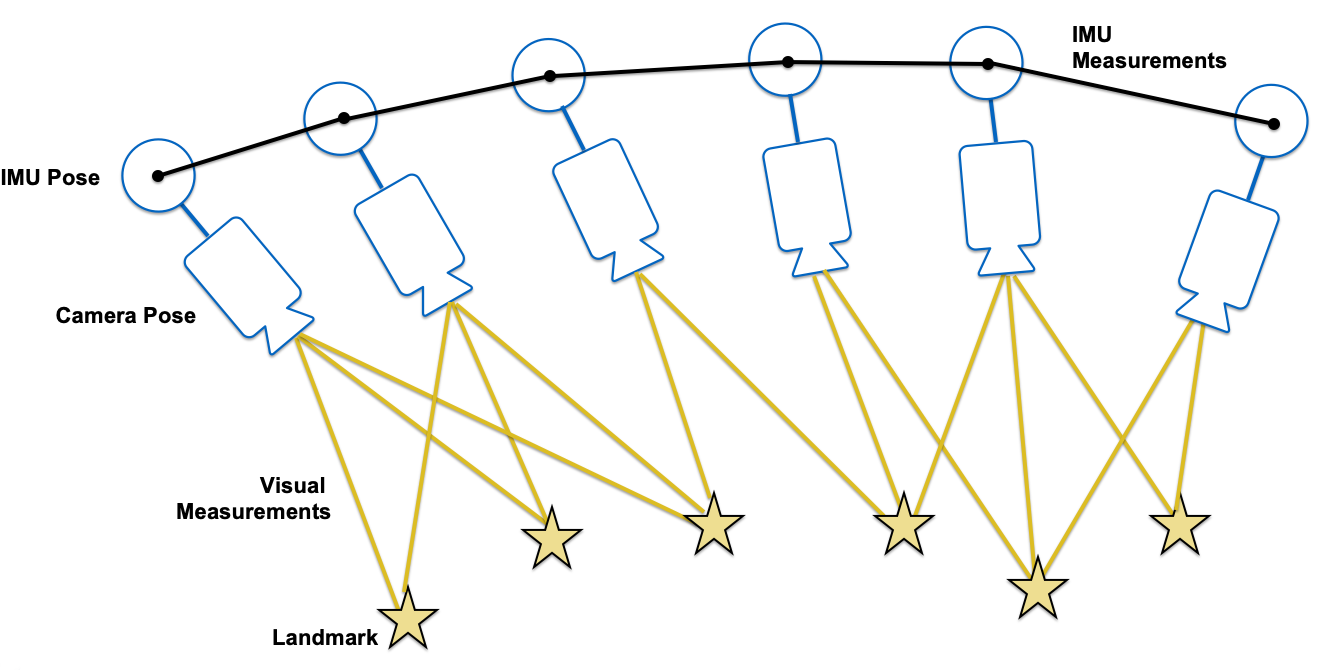
\includegraphics[width=\textwidth,height=\textheight,keepaspectratio]{../vio.png}
                    \caption{Visual IMU Odometry}
                \end{figure}
                ~\newline
                This module operates with inputs from the Simultaneous Localization and Mapping (SLAM) module, where sensor fusion for GPS, Inertial Measurement Unit (IMU), and Visual-Inertial Odometry (VIO) or Lidar-Inertial Odometry (LIO) has been applied. The final estimated location for the robot is obtained through SLAM, and based on this information, the module plans the next movement. 
                
            \paragraph{Inputs}
                ~\newline
                \begin{table}[H]
                  \centering
                    \caption{Input Variables of VIO or LIO Odometry with GPS} \label{tbl:Input Variables of VIO or LIO Odometry with GPS}
                  \begin{tabularx}{\textwidth}{|p{5cm}|p{2cm}|p{1.2cm}|p{1cm}|X|}
                    \hline Variable Name & Variable Type & Units & Range & Description \\
                    \hline m\_IMUReading & 2D list &  N/A & TBD & Output from last IMU reading.\\
                    \hline m\_GPSReading & 2D list &  N/A & TBD & Output from last GPS reading.\\
                    \hline m\_CameraReading & 2D list &  N/A & TBD & Output from last visual odometry reading compare to land.\\
                    \hline m\_CurrentSpeed  & float & $m/s$ & TBD & Current Speed of WBR\\
                    \hline m\_CurrentAcceleration & float & $m/s^2$ & TBD & Current Acceleration of WBR\\
                    \hline m\_CurrentRotation & 2D list & N/A & TBD & Current global Rotation in pitch yaw roll axis\\
                    \hline
                  \end{tabularx}
                \end{table} 
                
            \paragraph{Outputs}
                ~\newline
                \begin{table}[H]
                  \centering
                    \caption{Output Variables of VIO or LIO Odometry with GPS} 
                    \label{tbl:Output Variables of VIO or LIO Odometry with GPS}
                  \begin{tabularx}{\textwidth}{|p{5cm}|p{2cm}|p{1.2cm}|p{1cm}|X|}
                    \hline Variable Name & Variable Type & Units & Range & Description \\
                    \hline estimated location & 2D list &  N/A & TBD & Output from SLAM module that get estimation from sensor fusion.\\
                    \hline
                  \end{tabularx}
                \end{table}                 
            \paragraph{Exception Handling}
                ~\newline
                If any sensor does not got read or disconnected during movement. That sensor will be abundant from sensor fusion. 
                
            \paragraph{Timing Constraints}
                ~\newline
                This module need to be finished within 100ms as well which is the next reading will come up from sensors. 
                
            \paragraph{Initialization}
                ~\newline
                Set everything to zero. 
                
        \newpage
        \subsubsection{Simultaneous Localization and Mapping : Local Obstacle Update}
            \paragraph{Description}
                \begin{figure}[H]
                    \centering
                    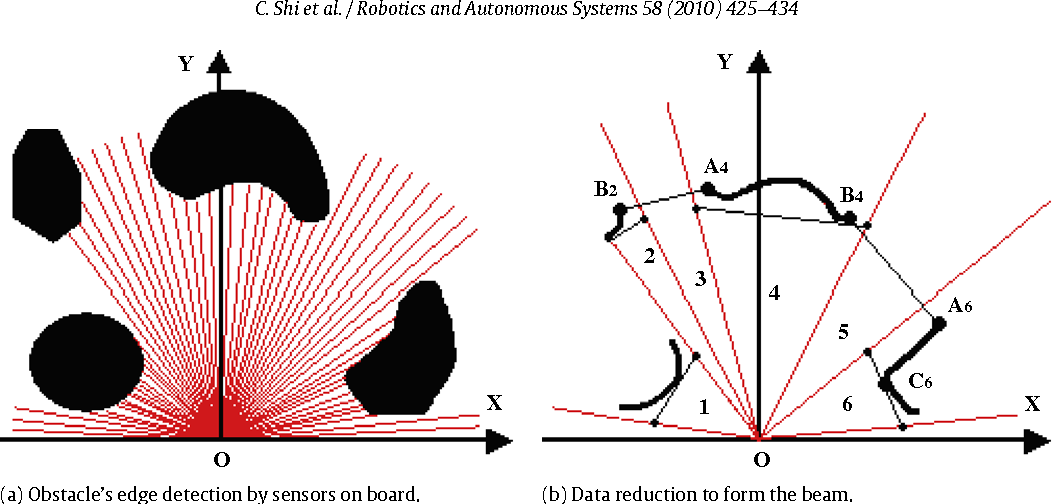
\includegraphics[width=\textwidth,height=\textheight,keepaspectratio]{../local_obstacle_avoidence.png}
                    \caption{Local Obstacle Avoidance}
                \end{figure}  
                ~\newline
                The Local Obstacle Update module is an integral component of the autonomous navigation system, tasked with continuously monitoring and updating the representation of obstacles within the immediate environment of the robot. This module operates in conjunction with sensors, such as lidar or cameras, to dynamically assess the surroundings and adapt the obstacle map in real-time. \\ 
            \paragraph{Inputs}
                ~\newline
                \begin{table}[H]
                  \centering
                    \caption{Input Variables of Local Obstacle Update} 
                    \label{tbl:Input Variables of Local Obstacle Update}
                  \begin{tabularx}{\textwidth}{|p{5cm}|p{1.2cm}|p{1.2cm}|p{1cm}|X|}
                    \hline Variable Name & Variable Type & Units & Range & Description \\
                    \hline c\_CurrentLocation & 2D list &  N/A & TBD & The current location WBR is at.\\
                    \hline m\_CameraReading & 2D list &  N/A & TBD & Output from last visual depth reading.\\
                    \hline current location & 2D list &  N/A & TBD & The current location WBR is at.\\
                    \hline m\_CurrentRotation & 2D list & N/A & TBD & Current global Rotation in pitch yaw roll axis\\
                    \hline
                  \end{tabularx}
                \end{table} 
            \paragraph{Outputs}
                ~\newline
                \begin{table}[H]
                  \centering
                    \caption{Output Variables of Local Obstacle Update} 
                    \label{tbl:Output Variables of Local Obstacle Update}
                  \begin{tabularx}{\textwidth}{|p{5cm}|p{1.2cm}|p{1.2cm}|p{1cm}|X|}
                    \hline Variable Name & Variable Type & Units & Range & Description \\
                    \hline c\_ObstaclesLocations & 2D list &  N/A & TBD & Collection of local obstacles locations in list.\\
                    \hline
                  \end{tabularx}
                \end{table}                     
            \paragraph{Exception Handling}
                ~\newline
                Obstacle that is on the way and too close will trigger emergency stop. And if obstacles are blocking entire possible path, it will also stop and wait for 5 mins. \\
                
            \paragraph{Timing Constraints}
                ~\newline
                This module need to run at the same time as the same speed as SLAM and local avoidance module. So it need to be finished in 100ms. \\
                
            \paragraph{Initialization}
                ~\newline
                Set everything to 0. \\
                
        \newpage
        \subsubsection{Simultaneous Localization and Mapping : Area Restriction}
            \paragraph{Description}
                \begin{figure}[H]
                    \centering
                    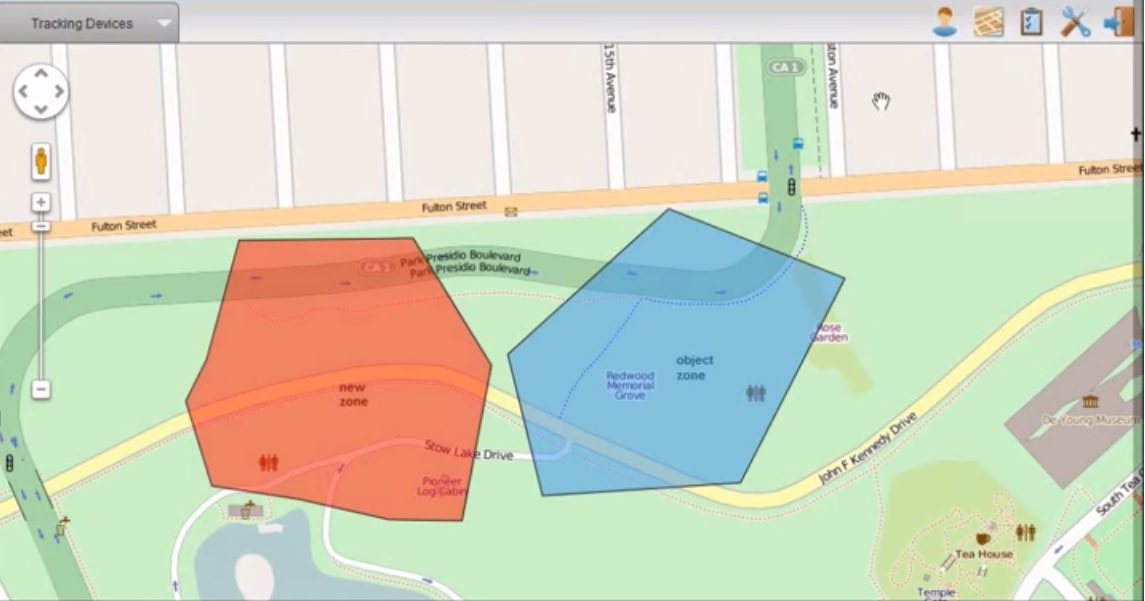
\includegraphics[width=\textwidth,height=\textheight,keepaspectratio]{../GeoFence.jpg}
                    \caption{Geo Fence}
                \end{figure}  
                ~\newline
                The Area Restriction module is designed to confine the movement of WBR  within predefined geographical boundaries. This module plays a crucial role in scenarios where it is essential to restrict the robot's access to specific areas, ensuring compliance with operational regulations or safety constraints. The primary function of this module is to monitor and control the robot's navigation, preventing it from entering restricted zones or areas with potential hazards.\\ 
            \paragraph{Inputs}
                ~\newline
                \begin{table}[H]
                  \centering
                    \caption{Input Variables of Area Restriction} 
                    \label{tbl:Input Variables of Area Restriction}
                  \begin{tabularx}{\textwidth}{|p{5cm}|p{1.2cm}|p{1.2cm}|p{1cm}|X|}
                    \hline Variable Name & Variable Type & Units & Range & Description \\
                    \hline c\_ROSMap & 2D List & N/A & TBD & Output that show all passable area.\\
                    \hline c\_GeoFence & 2D List & N/A & TBD & List and include all the point for geo boundaries.\\
                    \hline
                  \end{tabularx}
                \end{table} 
                
            \paragraph{Outputs}
                ~\newline
                \begin{table}[H]
                  \centering
                    \caption{Output Variables of Area Restriction} 
                    \label{tbl:Output Variables of Area Restriction}
                  \begin{tabularx}{\textwidth}{|p{5cm}|p{1.2cm}|p{1.2cm}|p{1cm}|X|}
                    \hline Variable Name & Variable Type & Units & Range & Description \\
                    \hline c\_ROSMap & 2D List & N/A & TBD & Output that show all passable area.\\
                    \hline
                  \end{tabularx}
                \end{table}
                
            \paragraph{Exception Handling}
                ~\newline
                Human correction will be applied for double check on the generated map. \\
                
            \paragraph{Timing Constraints}
                ~\newline
                Since this function runs right after map transformation and need human correction. So there is barely any time constraints for the generation pats. \\
            \paragraph{Initialization}
                ~\newline
                Gather information from map transformation module\\
                
    \subsection{Control Module} \label{sec:Control Module}
        The control module is the heart of the system as it will be the primary system to interact with the surroundings in real-time. It has major functions to perform depending on the input from the \acrshort{cv} system: Normal Movement Control and Jumping Control.\\\\
        As illustrated in figure \ref{fig:Control Module Decomposition.png}. Control system runs in a while loop that never stops until system shut down. For each loop, it runs Motion Planner, Forward Kinematics, Jump manager, and VMC modules in series. It also runs \acrshort{cv} interface module in parallel. 
        \begin{sidewaysfigure}
            \centering
            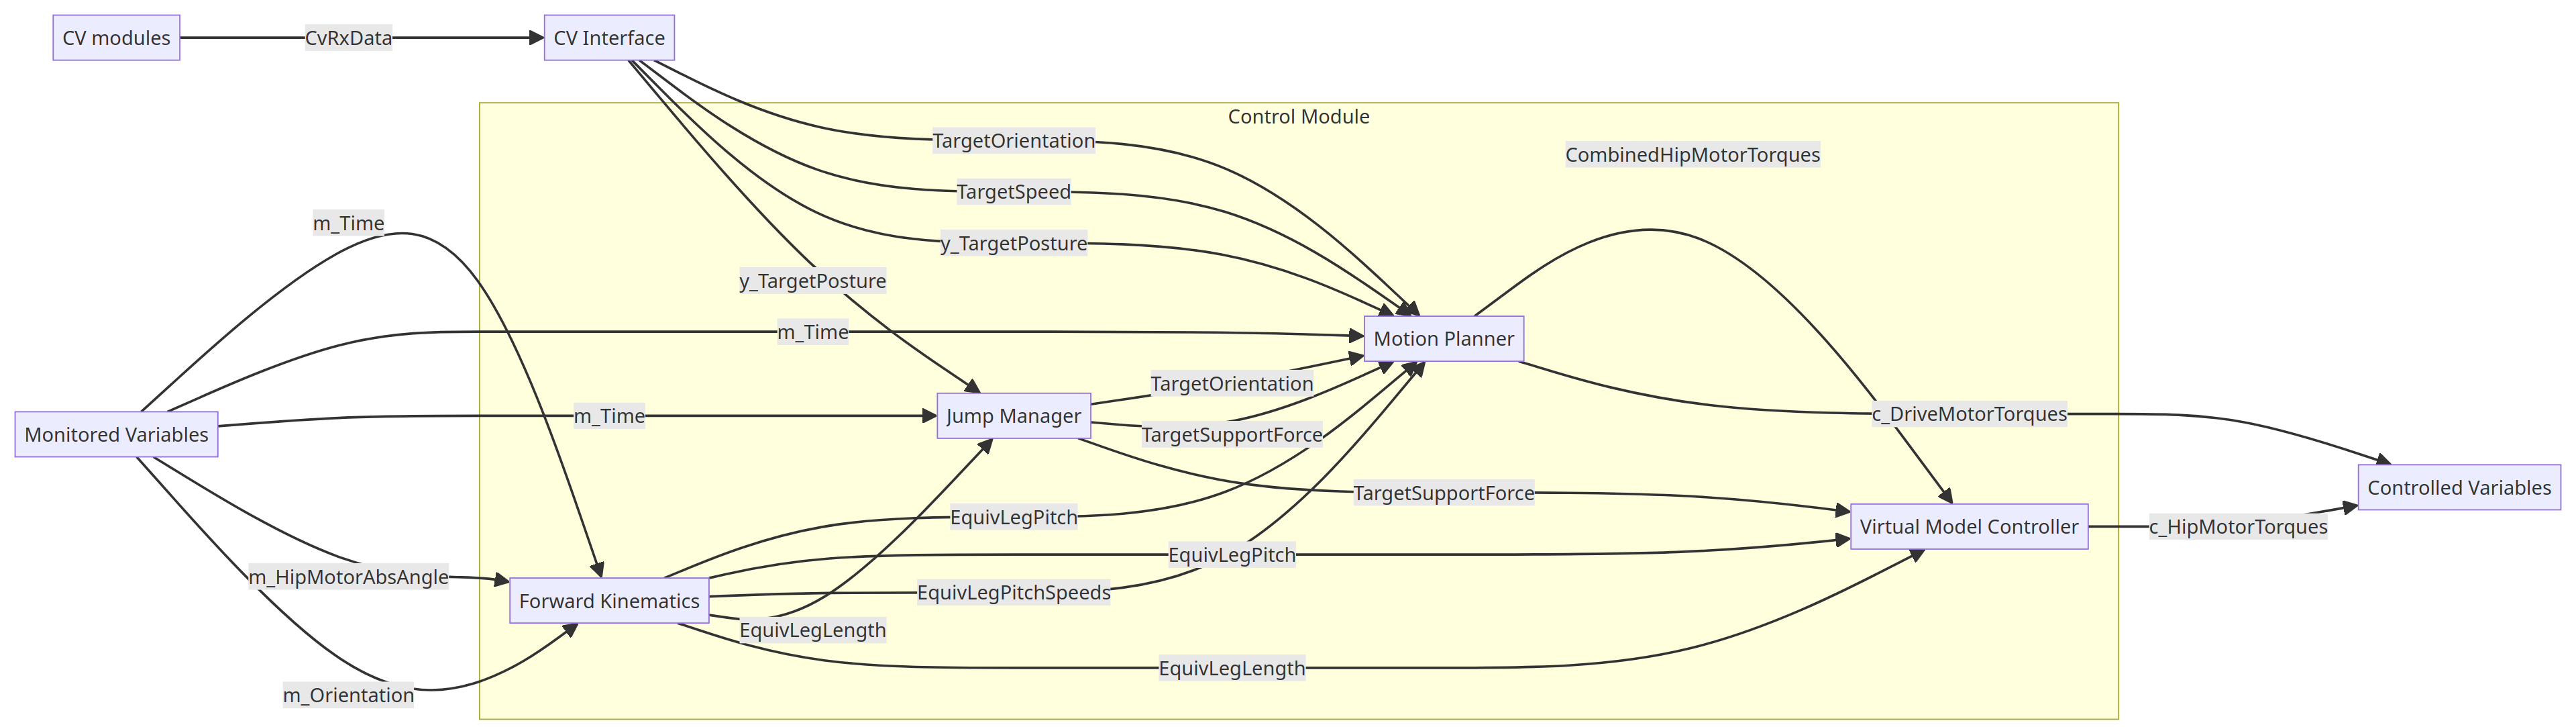
\includegraphics[width=\textwidth,height=\textheight,keepaspectratio]{../Control Module Decomposition.png}
            \caption{Control Model Decomposition}
            \label{fig:Control Module Decomposition.png}
        \end{sidewaysfigure}
            
        \subsubsection{Description}
            For normal situations when robot is moving on the ground, we used the open source code from \cite{HarbinEngWebotsGit2024}, whose system design is illustrated in \cite{HarbinEngCtrlDesign2022}. This section gives an overview of the open source design.\\\\
        
            \begin{figure}[H]
                \centering
                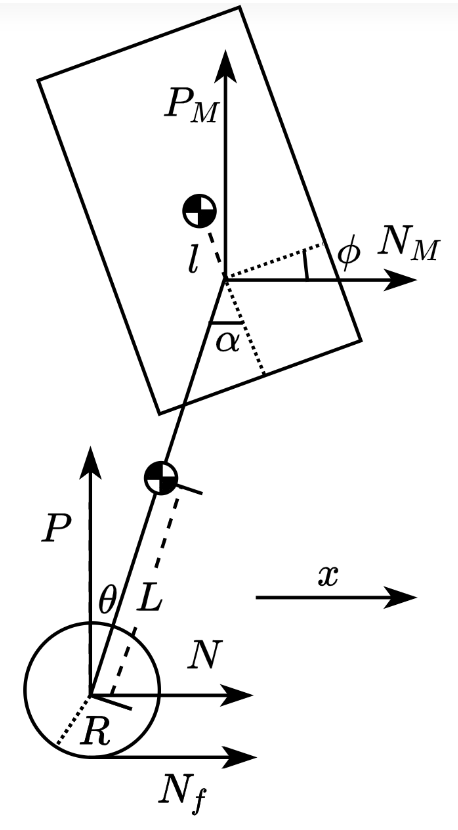
\includegraphics[width=\textwidth,height=\textheight-300pt,keepaspectratio]{../WBR Control Model Side View.png}
                \caption{WBR Control Model Side View, from \cite{HarbinEngCtrlDesign2022}}
                \label{fig:WBR Control Model Side View}
            \end{figure}

            The symbols shown in Figure \ref{fig:WBR Control Model Side View} are defined in table \ref{tbl:WBR Control Model Side View Symbols}. The supporting leg here is the segment connecting center of a side of the chassis to the wheel center and is called "equivalent leg". The preliminary assumption for normal movement analysis is that hip angle is fixed, so that length of this equivalent leg does not change, and we can apply inverted-pendulum model to let robot balance to stable position. Left and right side of the robot are calculated separately because they may have different leg length when operating.\\\\
            The main difference between normal movement control and jumping control is that the latter situation requires consideration of change in leg length. In normal movement control situation we will make sure change in leg lengths are slow that we can assume they are fixed at each time instance.
            
            \begin{table}[H]
                \begin{tabular}{|p{0.1\textwidth}|p{0.4\textwidth}|p{0.1\textwidth}|p{0.1\textwidth}|}
            
                    \hline Symbols   & Description & Positive Direction     & Unit        \\
                    \hline $ \theta$ & Angle between equivalent leg and vertical direction                            & As shown in the figure & rad         \\
                    \hline $ x     $ & Displacement in drive wheel                                                    & As shown in the figure & m           \\
                    \hline $ \phi  $ & Angle between robot body and horizontal direction                              & As shown in the figure & rad         \\
                    \hline $ T     $ & Output torque by drive motor                                                   & Same as $\theta$         & $N \cdot m$         \\
                    \hline $ T_p   $ & Combined output torque by the two hip motors                                   & Same as $\alpha$         & $N \cdot m$         \\
                    \hline $ N        $ & Horizontal portion of supporting force by drive wheel                          & As shown in the figure & N           \\
                    \hline $ P        $ & Vertical portion of supporting force by drive wheel                            & As shown in the figure & N           \\
                    \hline $ N_M      $ & Horizontal portion of supporting force by equivalent leg                       & As shown in the figure & N           \\
                    \hline $ N_f      $ & Friction force on drive wheel by the ground                                    & As shown in the figure & N           \\
            
                    \hline $ R  $      & Radius of drive wheel                                                          & N/A                    & m           \\
                    \hline $ L  $      & Distance from mass center of equivalent leg to drive wheel                     & N/A                    & m           \\
                    \hline $ L_M  $    & Distance from mass center of equivalent leg to rotational center of robot body & N/A                    & m           \\
                    \hline $ l  $      & Distance from mass center of robot body to rotational center of it             & N/A                    & m           \\
                    \hline $ m_w  $    & drive wheel mass                                                               & N/A                    & kg          \\
                    \hline $ m_p  $    & equivalent leg mass                                                            & N/A                    & kg          \\
                    \hline $ M  $      & Robot body mass                                                                & N/A                    & kg          \\
                    \hline $ I_w  $    & Rotational momentum of drive wheel around its mass center                      & N/A                    & $kg\cdot m^2$ \\
                    \hline $ I_p  $    & Rotational momentum of equivalent leg around its mass center                   & N/A                    & $kg\cdot m^2$ \\
                    \hline $ I_M  $    & Rotational momentum of robot body around its mass center                       & N/A                    & $kg\cdot m^2$ \\
            
                    \hline
                \end{tabular}
                \caption{WBR Control Model Side View Symbols} \label{tbl:WBR Control Model Side View Symbols}
            \end{table}

            And the following expressions describe our aggregated nonlinear system. x specifies all the control system inputs, and u specifies all the outputs.
            \[
                \vec{x}=\begin{bmatrix}\theta\\\dot{\theta}\\x\\ \dot{x}\\\phi\\ \dot{\phi}\\\end{bmatrix},\vec{u}=\begin{bmatrix}T\\T_p\\\end{bmatrix} ,\dot{\vec{x}}=f(\vec{x},\vec{u})
            \]
            
            Our objective is to let robot approach upright posture with zero torque to maintain in ideal situation.
            \[
                \vec{x}=\begin{bmatrix}0\\0\\x\\0\\0\\0\\\end{bmatrix},\vec{u}=\begin{bmatrix}0\\0\\\end{bmatrix}
            \]
            In order to approach this ideal state, the open source \cite{HarbinEngCtrlDesign2022} chose to use an \acrshort{lqr} controller, so do we. Because details are extensively stated on the referred website, it is not stated here. The main contribution of our project is to adapt this controller software to our specific hardware system, and also implement Jumping control to it. The main idea of the \acrshort{lqr} control is to construct system input to be,$\vec{u}=-K\vec{x}$, where the gain matrix K is calculated as an result of LQR optimization, based on given form of cost function, and it only depends on the equivalent leg length when robot is operating.\\\\
        
        \subsubsection{Inputs}
            \begin{table}[H]
              \centering
                \caption{Input Variables of General Control Module} \label{tbl:Input Variables of General Control Module}
              \begin{tabularx}{\textwidth}{|p{5cm}|p{1.5cm}|p{2cm}|p{2cm}|X|}
                \hline Variable Name & Variable Type & Units & Range & Description \\
                \hline m\_TargetRollAngle & Digital & m/s & -1 to 1 & Commanded roll angle of chassis platform by CV.\\
                \hline m\_TargetPitchAngle & Digital & m/s & -1 to 1 & Commanded roll angle of chassis platform by CV.\\
                \hline y\_Posture & Digital & N/A &\{e\_Jump, e\_Normal, \acrshort{tbd}\} & Commanded posture by CV.  \\
                \hline m\_TargetSpeed & Digital & m/s & -1 to 1 & Commanded velocity by CV.\\
                \hline m\_HipMotorAbsAngle & Digital Array & 0-max (TBD) & TBD & Encoder value of four hip motors\, measuring absolute angle.\\
                \hline m\_Orientation         & Analog Array  & \unit{\radian} & TBD & Orientation of chassis\, to be sensed by \acrshort{imu}\\
                \hline m\_Time & Digital & \unit{\second}  & TBD & Real-world time\\
                \hline
              \end{tabularx}
            \end{table}
        \subsubsection{Outputs}
            \begin{table}[H]
              \centering
                \caption{Output Variables of General Control Module} \label{tbl:Output Variables of General Control Module}
              \begin{tabularx}{\textwidth}{|p{5cm}|p{1.2cm}|p{1.2cm}|p{1cm}|X|}
                \hline Variable Name & Variable Type & Units & Range & Description \\
                \hline c\_DriveMotorTorques   & Digital Array & \unit{N.m} & TBD & Desired torque of drive motors \\
                \hline c\_HipMotorTorques     & Digital Array & \unit{N.m} & TBD & Desired torque of hip motors   \\
                \hline
              \end{tabularx}
            \end{table}
        \subsubsection{Internal Variables}
            \begin{table}[H]
              \centering
                \caption{Internal Variables of General Control Module} \label{tbl:Internal Variables of General Control Module}
              \begin{tabularx}{\textwidth}{|p{5.5cm}|p{1.5cm}|p{1.2cm}|p{2cm}|X|}
                \hline Variable Name & Variable Type & Units & Range & Description \\
                \hline EquivLegPitch & Digital Array & rad & TBD & Angle between equivalent left/right leg and horizontal direction. Calculated by forward Kinematics of figure \ref{fig:Leg Linkage}.\\
                \hline EquivLegPitchSpeeds & Digital Array & rad & TBD & Derivative of EquivLegPitch\\
                \hline DriveWheelDisplacements & Digital Array & rad & TBD & Ground displacement by drive wheels\\
                \hline DriveWheelSpeed & Digital & rad & TBD & Derivative of DriveWheelDisplacement\\
                \hline EquivLegLength & Digital Array & rad & TBD & Length of equivalent left/right legs\, which is distance from rotational center of robot body to drive wheel\\
                \hline PrevTime & Digital & s & TBD & Time at previous interrupt\\
                \hline
              \end{tabularx}
            \end{table}
            
        \subsubsection{Exception Handling}
            Input and output validation will be the main form of exception handling. All mandatory values will be checked to ensure they are not empty, and not out of specified limit. If any input or output is out of specified limit, encapsulate it to the maximum or minimum.\\\\
            In addition, if pitch of robot body, i.e. $m\_\phi$, is greater than a value, all motors shall be shut down to prevent undetermined damage when system has tripped over.
        \subsubsection{Timing Constraints} \label{sec:Control Module Timing Constraints}
            Operate as fast as possible so that velocity measurement can be as precise as possible. This is the highest priority task of control board.
        \subsubsection{Initialization}
            Reset all variables to zero.

    \subsection{Control Submodule: Forward Kinematics Module}
        \subsubsection{Description}
            Convert hip motor angles to end-effector (drive motor) configurations according to figure \ref{fig:Leg Linkage}.
            
        \subsubsection{Inputs}
            \begin{table}[H]
              \centering
                \caption{Input Variables of Forward Kinematics Module} \label{tbl:Input Variables of Forward Kinematics Module}
              \begin{tabularx}{\textwidth}{|p{5cm}|p{1.2cm}|p{1.2cm}|p{1cm}|X|}
                \hline Variable Name & Variable Type & Units & Range & Description \\
                \hline m\_HipMotorAbsAngle & Digital Array & 0-max (TBD) & TBD & Encoder value of four hip motors\, measuring absolute angle.\\
                \hline m\_Orientation         & Analog Array  & \unit{\radian} & TBD & Orientation of chassis\, to be sensed by \acrshort{imu}\\
                \hline m\_Time & Digital & \unit{\second}  & TBD & Real-world time\\
                \hline
              \end{tabularx}
            \end{table}
            
        \subsubsection{Outputs}
            \begin{table}[H]
              \centering
                \caption{Output Variables of Forward Kinematics Module} \label{tbl:Output Variables of Forward Kinematics Module}
              \begin{tabularx}{\textwidth}{|p{6cm}|p{1.2cm}|p{1.2cm}|p{1cm}|X|}
                \hline Variable Name & Variable Type & Units & Range & Description \\
                \hline EquivLegPitch & Digital & rad & TBD & Angle between equivalent leg and horizontal direction. $\phi_0$ in figure \ref{fig:Leg Linkage}.\\
                \hline EquivLegPitchVelocity & Digital & rad & TBD & Derivative of EquivLegPitch\\
                \hline EquivLegLength & Digital Array & rad & TBD & Length of equivalent left/right legs\, which is distance from rotational center of robot body to drive wheel\\
                \hline
              \end{tabularx}
            \end{table}
            
        \subsubsection{Exception Handling}
            Input and output validation will be the main form of exception handling. All mandatory values will be checked to ensure they are not empty, and not out of specified limit. If any input or output is out of specified limit, encapsulate it to the maximum or minimum.
        \subsubsection{Timing Constraints}
            Same as section \ref{sec:Control Module Timing Constraints}.
        \subsubsection{Initialization}
            Reset all input variables to zero.
        
    \subsection{Control Submodule: Jump Manager} \label{sec:Jump Manager}
        \subsubsection{Description}
            Jump Manager dynamically change control strategy and parameters to perform jumping action once commanded by the decision-making modules. This module is established to monitor the physical state of WBR and the real world time to govern the jumping procedure of WBR. The ultimate goal is to execute a safe and effective jump that significantly contributes to the robot's travel. The figure \ref{fig:Jump FSM} shows the whole process of jump action of WBR, including the process before it receives the jump command and after if fully completes the jump action and resumes initial position.\\\\
            \begin{figure}[H]
                \centering
                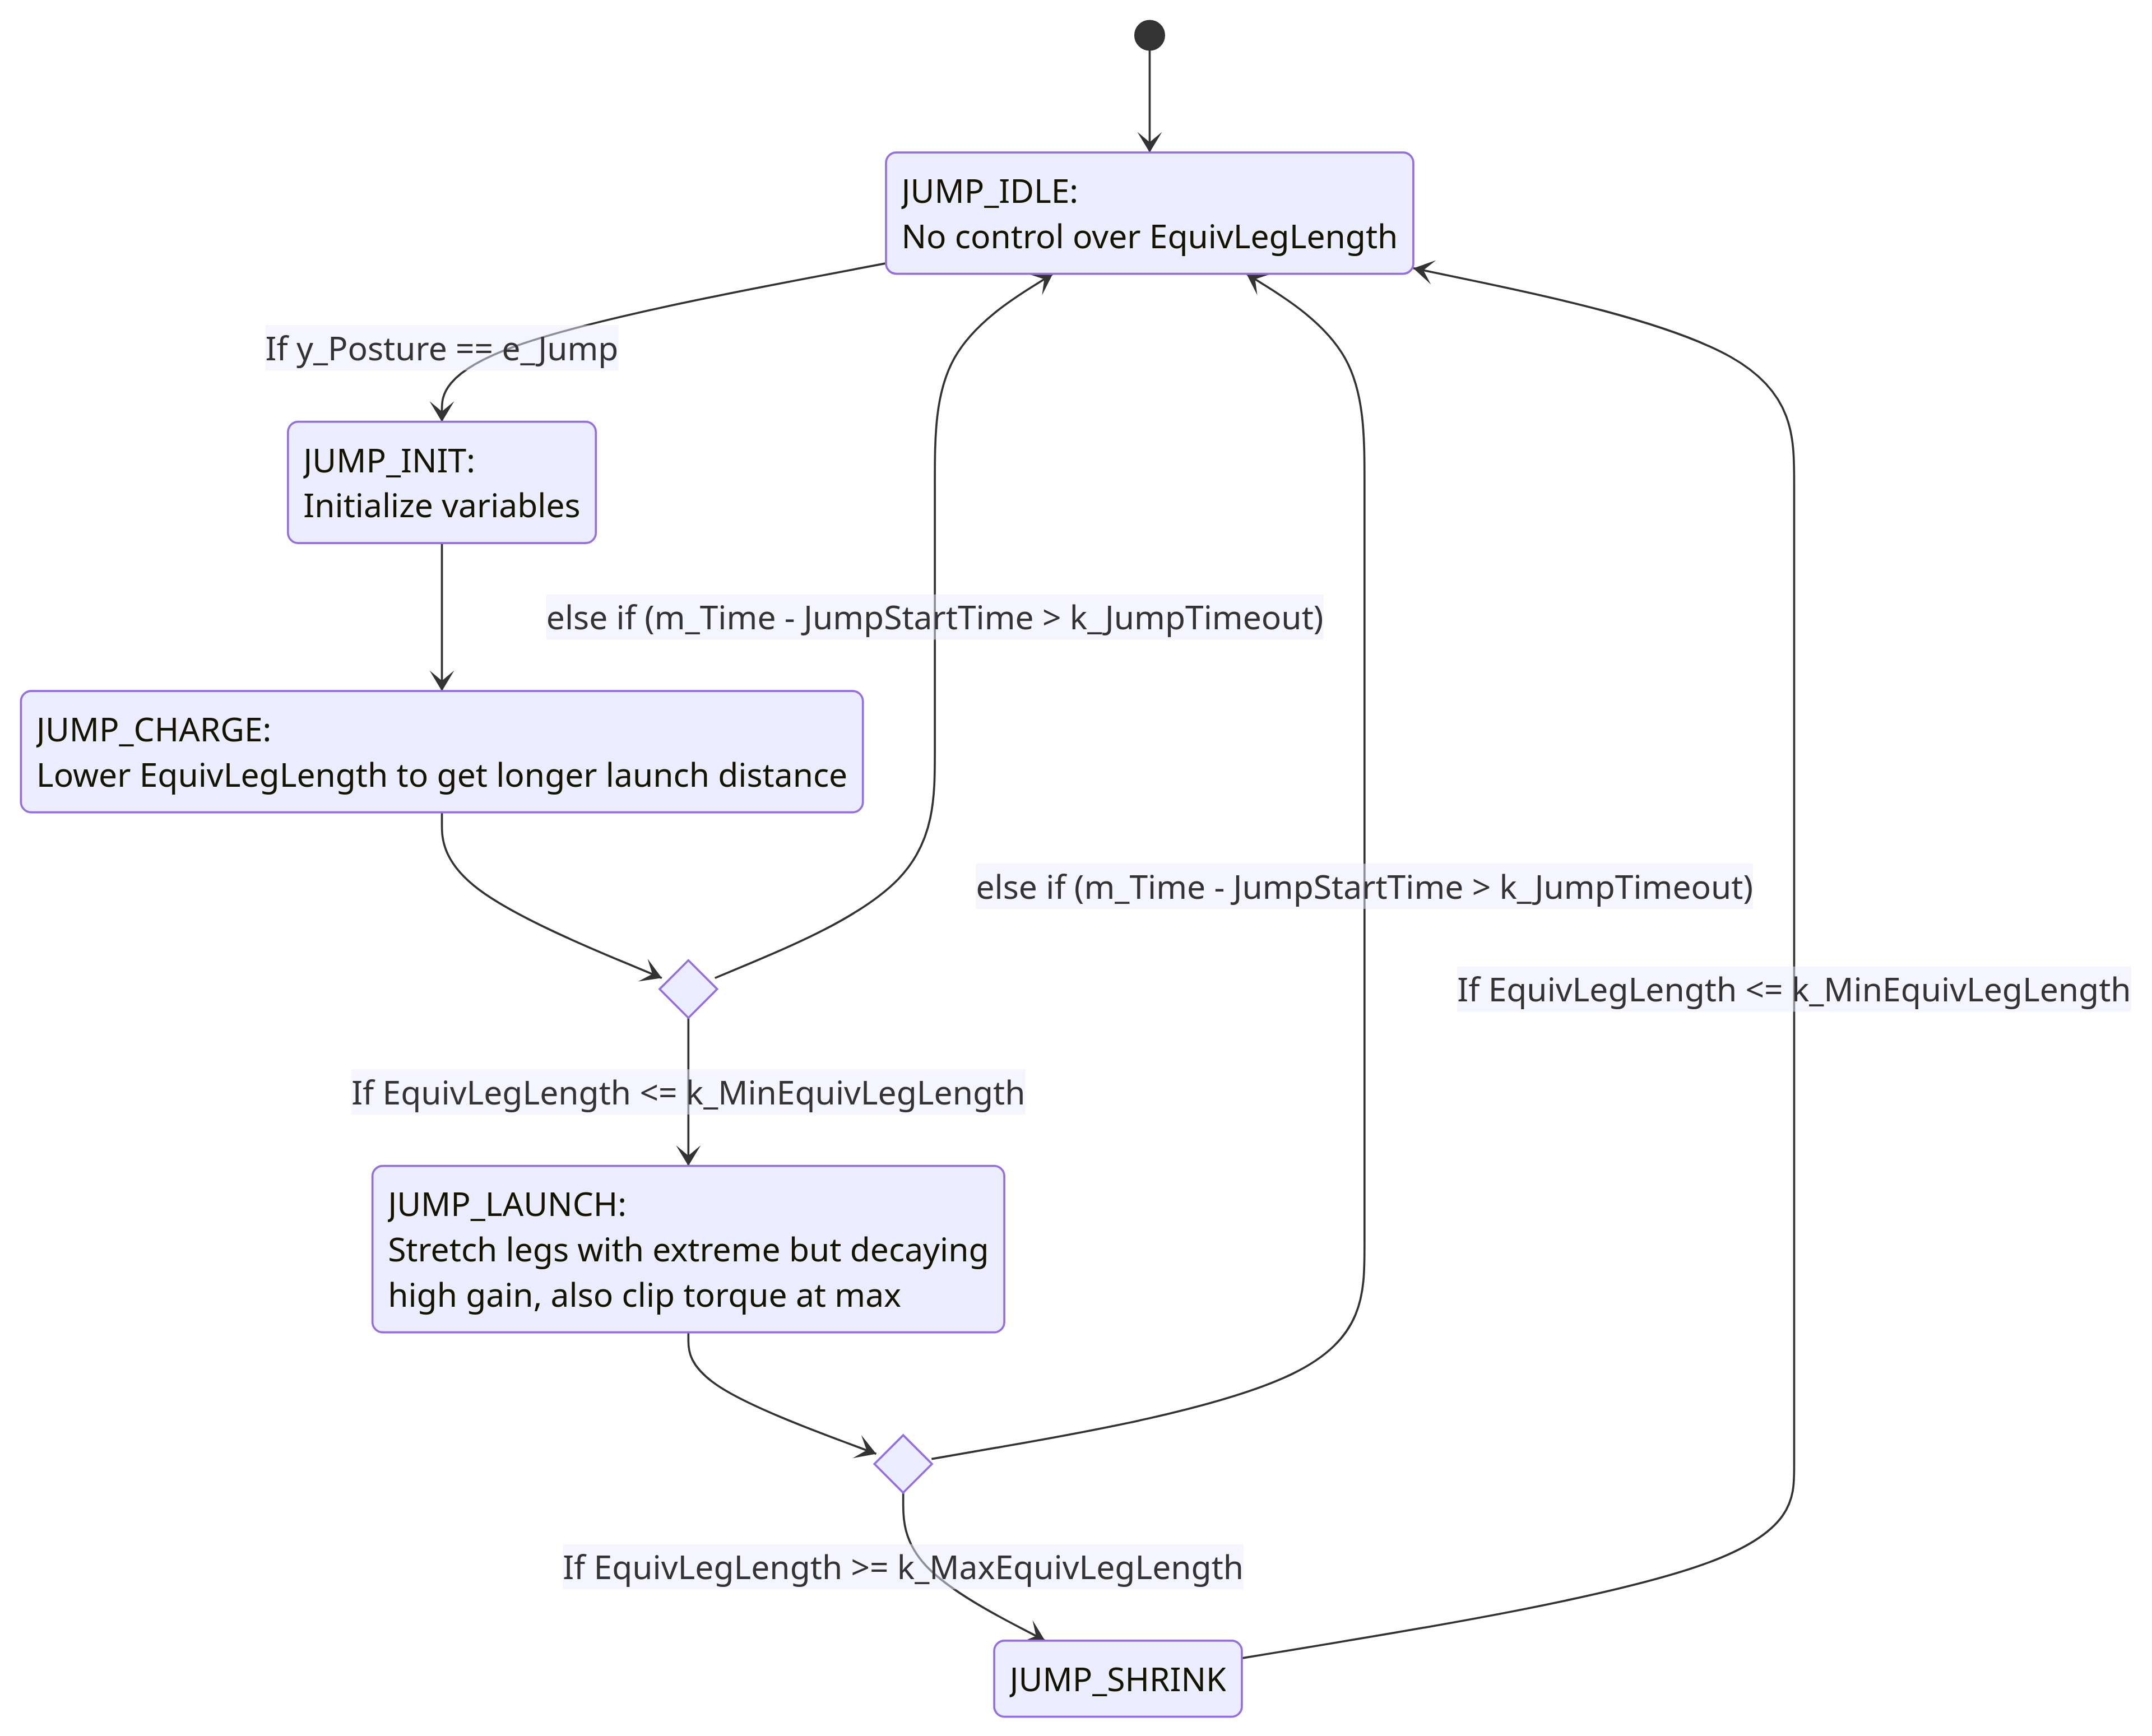
\includegraphics[width=\textwidth,height=\textheight,keepaspectratio]{../Jump FSM.png}
                \caption{Jump \acrshort{fsm}}
                \label{fig:Jump FSM}
            \end{figure}
        \subsubsection{Jump State Descriptions}
            Before WBR receives any jump command, it stays in JUMP\_IDLE state meaning it has nothing to do with jump process at the moment. Once there is a jump command, it starts to prepare and initialize all the variables that required to monitor and control during the jump action. By inputting \textbf{m\_Time}, the system continuously checking if in each state, the elapse time is greater than \textbf{k\_JumpTimeout}, which represents the maximum allowable duration for the jump action. This precautionary measure ensures that the system avoids being caught in an error state. By inputting and monitoring the variable \textbf {EquivLegLength} to take this physical state of WBR as a reference to deduce which stage the robot is in. To compare the \textbf {EquivLegLength} with the lowest acceptable height CoM, it can be inferred that if the robot finishes charging energy and will need to stretch legs and increase \textbf{c\_DriveMotorTorques} and \textbf {c\_HipMotorTorques} for a jump. To compare \textbf{EquivLegLength} with \textbf{k\_MinEquivLegLength}, the system will determine whether to decrease \textbf{c\_DriveMotorTorques} and \textbf{c\_HipMotorTorques} to bring the WBR back to a horizontal position.\\\\
            \textbf{JUMP\_IDLE:} WBR stays idle when there is no command received.\\\\
            \textbf{JUMP\_CHARGE:} WBR lower the \acrshort{com} to a predetermined level for the purpose of getting a longer launch distance. This primarily aimed at accumulating more energy for a higher jump. It is important to ensure CoM remains within the robot's bearing capacity, and it should not exceed the lowest acceptable CoM level.\\\\
            \textbf{JUMP\_LAUNCH:} Stretching legs but with decaying gain. The intentional reduction in gain serves as a buffer, mitigating large torques to prevent potential damage to the components.\\\\
            \textbf{JUMP\_SHRINK:} Lower CoM to its initial position.     
        \subsubsection{Inputs}        
            \begin{table}[H]
              \centering
                \caption{Input Variables of Jumping Control Module} \label{tbl:Input Variables of Jumping Control Module}
              \begin{tabularx}{\textwidth}{|p{3cm}|p{1.2cm}|p{1.1cm}|p{1.5cm}|X|}
                \hline Variable Name & Variable Type & Units & Range & Description \\
                \hline m\_Time & Digital & \unit{\second}  & TBD & Real-world time\\                
                \hline EquivLegLength & Digital Array & rad & TBD & Length of equivalent legs of left and right side\, which is distance from rotational center of robot body to drive wheel\\
                \hline y\_TargetPosture & Digital & N/A &\{e\_Jump, e\_Normal, \acrshort{tbd}\} & Commanded target posture state of robot  \\
                \hline
              \end{tabularx}
            \end{table}
        
        \subsubsection{Outputs} 
            \begin{table}[H]
                \centering
                \caption{Output Variables of Jumping Control Module} \label{tbl:Output Variables of Jumping Control Module}
                  \begin{tabularx}{\textwidth}{|p{4cm}|p{1.5cm}|p{1.25cm}|p{1cm}|X|}
                    \hline Variable Name & Variable Type & Units & Range & Description \\
                    \hline TargetOrientation & Digital Array  & rad & TBD & Commanded target orientation of chassis\\
                    \hline TargetSupportForce & Digital Array & N & TBD & Array of desired force and momentum going to apply to each leg\\
                    \hline                        
             \end{tabularx}
            \end{table}
        \subsubsection{Internal Variables}
            \begin{table}[H]
              \centering
                \caption{Internal Variables of Jumping Control Module} \label{tbl:Internal Variables of Jumping Control Module}
              \begin{tabularx}{\textwidth}{|p{5.5cm}|p{1.2cm}|p{1.2cm}|p{1cm}|X|}
                \hline Variable Name & Variable Type & Units & Range & Description \\
                \hline IsJumpTheAir & Boolean & N/A &N/A &  Indicating WBR is currently in the air or not.\\
                \hline JumpState &Enum &N/A &N/A & representing the current state of the jump procedure\\
                \hline PrevTime & Digital & s & TBD & Time at previous interrupt\\
                \hline
              \end{tabularx}
            \end{table}

        \subsubsection{Exception Handling}
            Input and output validation will be the main form of exception handling. All mandatory values will be checked to ensure they are not empty, and not out of specified limit. If any input or output is out of specified limit, encapsulate it to the maximum or minimum.\\\\
            Input variables will be checked if they are in the correct data type, as specified in the table above. If any of the data type is wrong, the system promptly reports the discrepancy as an issue.
        \subsubsection{Timing Constraints}
            Operate as fast as possible so that jump stage control can be as precise as possible.
        \subsubsection{Initialization}
            Reset all variables to zero.

    \subsection{Control Submodule: Motion Planner Module}
        \subsubsection{Description}      
            \begin{figure}[H]
                \centering
                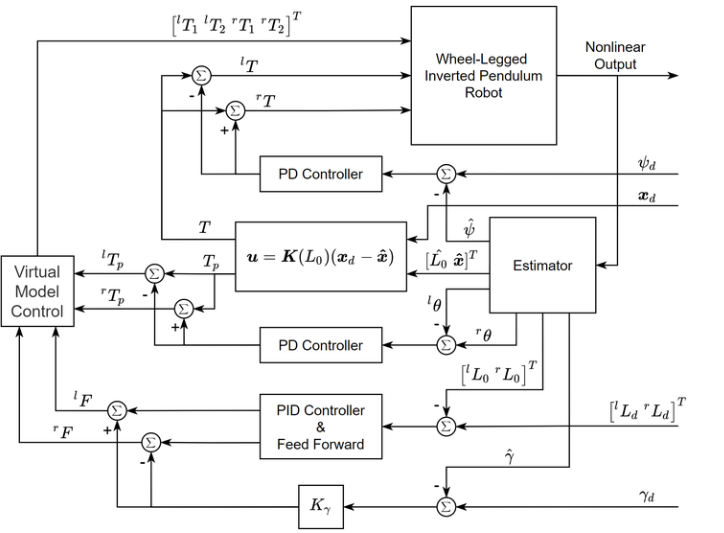
\includegraphics[width=\textwidth,height=\textheight,keepaspectratio]{../Motion Planner Design.png}
                \caption{Motion Planner Design from \citet{HarbinEngCtrlDesign2022}}
                \label{fig:Motion Planner Design}
            \end{figure}

            \begin{table}[H]
                \centering
                \begin{tabular}{|p{0.1\textwidth}|p{0.4\textwidth}|p{0.1\textwidth}|}            
                    \hline Symbols   & Description & Unit        \\
                    \hline $\phi_d$ & Robot body pitch target angle & rad \\            
                    \hline $\gamma_d$ & Robot body roll target angle & rad \\
                    \hline $[\leftindex^l {\theta},\leftindex^r {\theta}]$ & EquivLegPitch & rad \\
                    \hline $ T     $ & Output torque by drive motor & N*m         \\
                    \hline $ T_p   $ & Combined output torque by the two hip motors & N*m         \\
                    \hline $x_d$ & Current system status (main input) & N/A \\
                    \hline $[\leftindex^l {L}_b,\leftindex^r {L}_b]$ & Current left and right equivalent leg length\, provided by forward kinematics & m \\            
                    \hline
                \end{tabular}
                \caption{Main Symbols in Motion Planner Design} \label{tbl:Main Symbols in Motion Planner Design}
            \end{table}

            Integration of motion planner and \acrshort{vmc} is shown in Figure \ref{fig:Motion Planner Design}. We directly use the control system implemented by \citet{HarbinEngCtrlDesign2022}, so here we only give an overview.\\\\
            The estimator observes the \acrshort{ivp} plant and provides current system status to the controllers. Three \acrshort{pid} controller takes care of slight adjustment to the pitch and roll angle of robot body, and angle difference between left and right equivalent legs, respectively. The target for angle difference between equivalent legs is always set to zero.\\\\
            The main \acrshort{lqr} block, $\vec{u}=K(L_0)(\vec{x_d}-\vec{\hat{x}})$, constructs the output u as a linear combination of input x, where the gain is dependent on the equivalent leg length. Its outputs, planned drive motor torques and combined hip motor torques are passed into IVP and VMC for further control, respectively. VMC converts combined hip motor torques into individual hip motor torques. IVP directly outputs the drive motor torques.
        \subsubsection{Inputs}
            \begin{table}[H]
              \centering
                \caption{Input Variables of Motion Planner} \label{tbl:Input Variables of Motion Planner}
              \begin{tabularx}{\textwidth}{|p{5cm}|p{1.2cm}|p{1.2cm}|p{1cm}|X|}
                \hline Variable Name & Variable Type & Units & Range & Description \\
                \hline m\_Time & Digital & \unit{\second}  & TBD & Real-world time\\
                \hline m\_HipMotorAbsAngle & Digital Array & 0-max (TBD) & TBD & Encoder value of four hip motors\, measuring absolute angle.\\
                \hline m\_Orientation         & Analog Array  & \unit{\radian} & TBD & Orientation of chassis\, to be sensed by \acrshort{imu}\\
                \hline EquivLegPitch & Digital & rad & TBD & Angle between equivalent leg and horizontal direction. $\phi_0$ in figure \ref{fig:Leg Linkage}.\\
                \hline EquivLegPitchSpeeds & Digital Array & rad & TBD & Derivative of EquivLegPitch\\
                \hline 
              \end{tabularx}
            \end{table}        
            
        \subsubsection{Outputs} 
         \begin{table}[H]
                  \centering
                \caption{Output Variables of Motion Planner} \label{tbl:Output Variables of Motion Planner}
                  \begin{tabularx}{\textwidth}{|p{6cm}|p{1.5cm}|p{1.25cm}|p{1cm}|X|}
                    \hline Variable Name & Variable Type & Units & Range & Description \\
                    \hline c\_DriveMotorTorques   & Digital Array & \unit{N.m} & TBD & Desired torque of drive motors \\
                    \hline CombinedHipMotorTorques     & Digital Array & \unit{N.m} & TBD & Desired combined torque of hip motors   \\
                    \hline                        
             \end{tabularx}
            \end{table}
        \subsubsection{Internal Variables}
            \begin{table}[H]
              \centering
                \caption{Internal Variables of Motion Planner} \label{tbl:Internal Variables of Motion Planner}
              \begin{tabularx}{\textwidth}{|p{6cm}|p{1.2cm}|p{1.2cm}|p{1cm}|X|}
                \hline Variable Name & Variable Type & Units & Range & Description \\
                \hline DriveWheelDisplacements & Digital Array & rad & TBD & Ground displacement by drive wheels\\
                \hline DriveWheelSpeed & Digital & rad & TBD & Derivative of DriveWheelDisplacement\\
                \hline EquivLegLength & Digital Array & rad & TBD & Length of equivalent left/right legs\, which is distance from rotational center of robot body to drive wheel\\
                \hline PrevTime & Digital & s & TBD & Time at previous interrupt\\
                \hline
              \end{tabularx}
            \end{table}
        
        \subsubsection{Exception Handling}
            Input and output validation will be the main form of exception handling. All mandatory values will be checked to ensure they are not empty, and not out of specified limit. If any input or output is out of specified limit, encapsulate it to the maximum or minimum.\\\\
            Input variables will be checked if they are in the correct data type, as specified in the table above. If any of the data type is wrong, the system promptly reports the discrepancy as an issue.
        \subsubsection{Timing Constraints}
            Operate as fast as possible so that motion planning can be as precise as possible.
        \subsubsection{Initialization}
            Reset all variables to zero.
        
    \subsection{Control Submodule: VMC Module}
        \subsubsection{Description}            
            \acrfull{vmc} is a motion control language that uses simulations of imagined mechanical components to create forces, which are applied through real joint torques, thereby creating the illusion that the virtual components are connected to the robot, \cite{VmcForBiped}. For our particular use, \acrshort{vmc} converts combined hip motor torques into individual hip motor torques. It controls the system with the assumption of ideal virtual model as shown in figure \ref{fig:Leg Linkage}, and we shall apply the static force transformation formula $\vec{\tau}=J^T F$ to left and right side of the robot separately, where $\tau$ consists of desired front and back hip motor torques. Note that we have to assume acceleration and speed of all links are small enough to ignore. Derivation of the theorem can be found in chapter 5.10 of \cite{siciliano2009robotics}. $J^T$ is transpose of Jacobian matrix of linkage configuration, and F consists of desired external forces and momentum to generate, which are supporting force and momentum on the drive wheel end of equivalent leg.
        \subsubsection{Inputs}
             \begin{table}[H]
              \centering
                \caption{Input Variables of VMC Module} \label{tbl:Input Variables of VMC Module}
                \begin{tabularx}{\textwidth}{|p{5cm}|p{2cm}|p{1.2cm}|p{1cm}|X|}
                \hline Variable Name & Variable Type & Units & Range & Description \\
                \hline CombinedHipMotorTorques     & Digital Array & \unit{N.m} & TBD & Desired combined torque of hip motors   \\
                \hline TargetSupportForce & Digital array & N & TBD & Array of desired force and momentum going to apply to each leg.\\
                \hline EquivLegPitch & Digital Array & rad & TBD & Angle between equivalent left/right leg and horizontal direction. Calculated by forward Kinematics of figure \ref{fig:Leg Linkage}.\\
                \hline EquivLegLength & Digital Array & rad & TBD & Length of equivalent left/right legs\, which is distance from rotational center of robot body to drive wheel\\
                \hline 
              \end{tabularx}
            \end{table}
        
        \subsubsection{Outputs}
            \begin{table}[H]
              \centering
                \caption{Output Variables of VMC Module} \label{tbl:Output Variables of VMC Module}
                \begin{tabularx}{\textwidth}{|p{5cm}|p{2cm}|p{1.2cm}|p{1cm}|X|}
                \hline Variable Name & Variable Type & Units & Range & Description \\
                \hline c\_HipMotorTorques & Digital Array & $ N \cdot m $ & TBD & Desired torques of hip motors   \\
                \hline 
              \end{tabularx}
            \end{table}  
        
        \subsubsection{Exception Handling}
            Input and output validation will be the main form of exception handling. All mandatory values will be checked to ensure they are not empty, and not out of specified limit. If any input or output is out of specified limit, encapsulate it to the maximum or minimum.\\\\
            Input variables will be checked if they are in the correct data type, as specified in the table above. If any of the data type is wrong, the system promptly reports the discrepancy as an issue.
        \subsubsection{Timing Constraints}
            Operate as fast as possible so that it does not block other control sub-modules by much.
        \subsubsection{Initialization}
            Reset all variables to zero.
    
    \subsection{CV Interface Module}
        \subsubsection{Description}
            \acrshort{cv} Interface is the custom communication interface between \acrshort{cv} and control board designed by us. We choose to use the 1 Mbps \acrshort{uart}. This section explains our custom communication protocol. All the code, detailed implementation, and explanation are recorded in \cite{CvInterfaceGit2023}.\\\\
            The figure \ref{fig:CV Interface General Sequence Diagram} shows the general sequence CV and control board will follow to establish a communication session, synchronize timestamp, exchanging miscellaneous information, and communicating with robot movement (auto-move) and camera gimbal rotation (auto-aim) decisions. The camera gimbal rotation feature may not be implemented in this project, since it depends on whether we have time to add the camera gimbal module. If the mechanical structure of camera gimbal is not going to be added, we will fix the camera to the chassis platform.The drawback is the data input will not be stable for SLAM to process, but it is good enough for this project.\\\\
            
            Design ideas of the sequence diagram in figure \ref{fig:CV Interface General Sequence Diagram}:
            \begin{itemize}
                \item Unit of all timestamps is ms, format is uint16\_t. It's defined by timestamp = raw\_timestamp - sync\_time. if raw\_timestamp overflow and becomes smaller than sync\_time, timestamp = raw\_timestamp - sync\_time + 0x10000 to avoid negative number. Exception are TranDelta and TranDelta\_MA, which are int16\_t, because it may become negative when control board's tick updates slower than CV
                \item Reason for CV to request for CvSyncTime at around the 8th step: CV may send multiple ACKs to multiple set-mode requests that are stuck in the buffer before CV starts processing. CV will memorize the CvSyncTime of the last ACK, while control board may not, since some messages may be lost caused by turn around time of DMA controller. Therefore, to correlate, control board must have latest CvSyncTime stored and sent to CV when requested
                \item TranDelta history should be cleared every time Control board boots up.
                \item For consistency, all timestamps within package headers should be synchronized, i.e. offseted by SyncTime, even before the synchronization process, where . For example, for control board, the timestamp should be CtrlTimestamp(Tx) - CtrlSyncTime. For CV, the timestamp should be CvTimestamp(Tx) - CvSyncTime.
                \item For all msgs control receives from CV, update TranDelta\_MA and its history. Newest TranDelta = CtrlTimestamp(Rx) - CtrlSyncTime - MsgTimestamp, except for the ACK msg where calculation is different as illustrated in the diagram below
            \end{itemize}
            
            \begin{figure}[H]
                \centering
                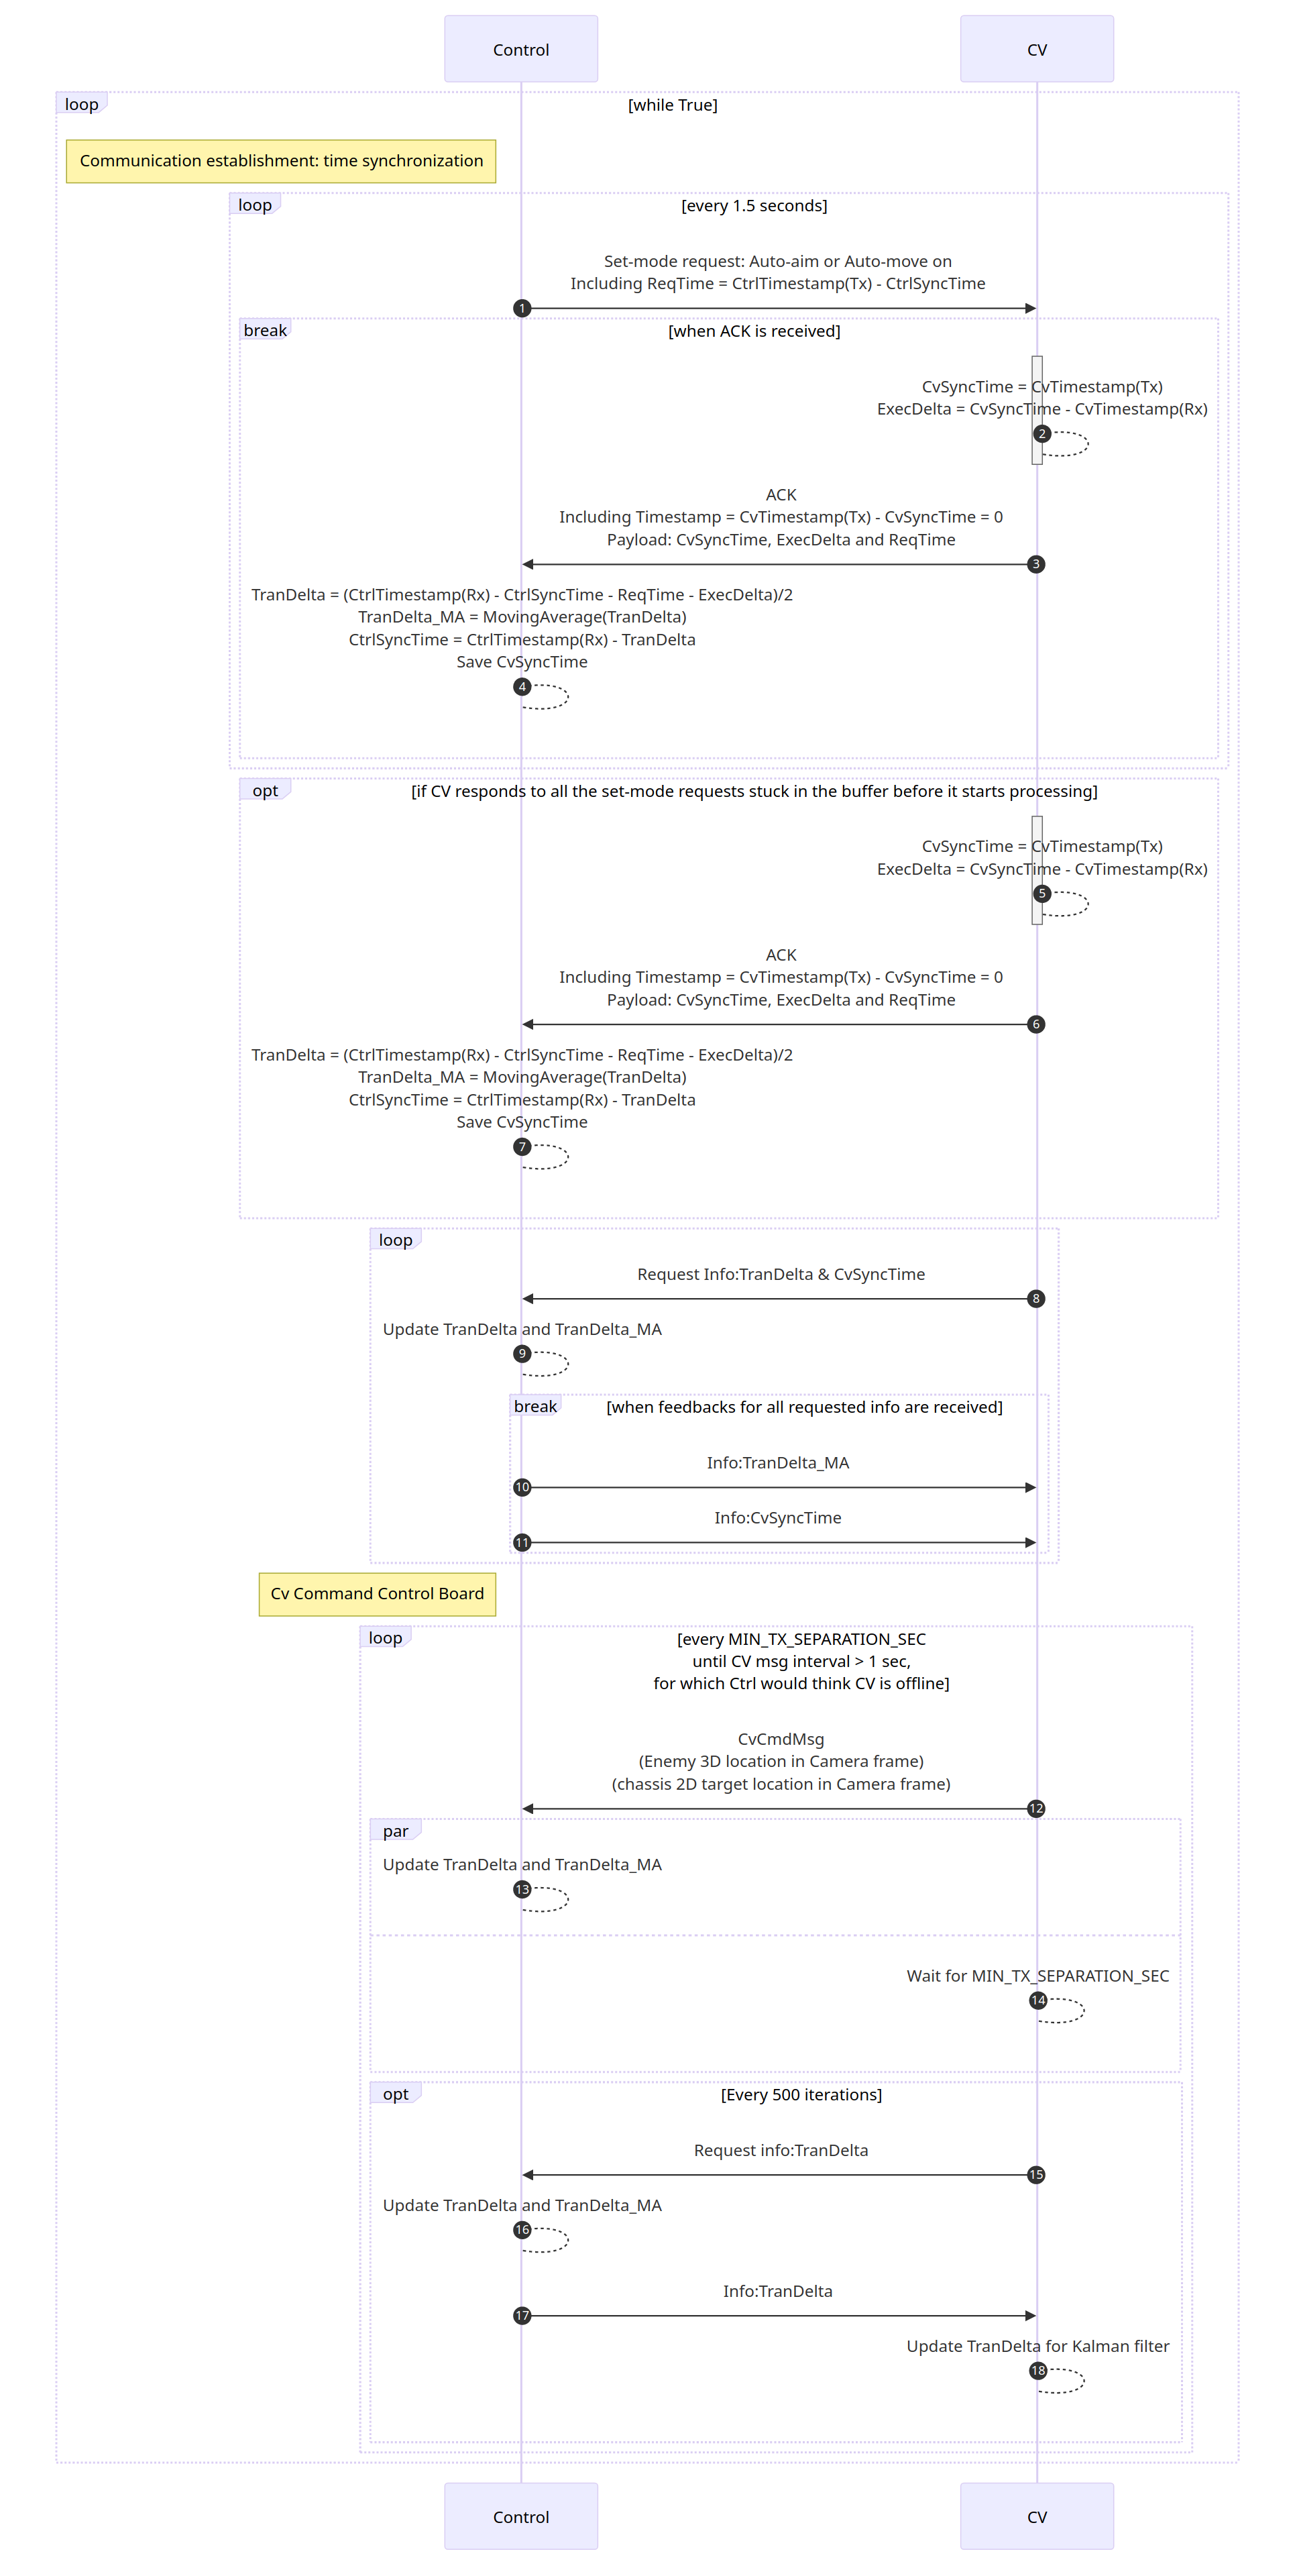
\includegraphics[width=\textwidth,height=\textheight,keepaspectratio]{../CV Interface General Sequence Diagram.png}
                \caption{CV Interface General Sequence Diagram}
                \label{fig:CV Interface General Sequence Diagram}
            \end{figure}
            Individual package format will be recorded in \cite{CvInterfaceGit2023}, and it will not be included here for convenience. However, the general data structure is shown in table \ref{tbl:CV Interface Data Frame}. To reduce processor work load of control board being interrupted at each incoming bit and the end of each packet, all packet types are designed to have the same size, and unused data field are to padded with 0xFF for package validation. With fixed package size, the control board can use \acrshort{dma} controller that processes the individual bit transmission in the background.\\\\
            The timestamp field in each package is used to identify the unavoidable control loop delay, so that the control system can predict the intended target action based on the delayed and received command from CV.
            \begin{table}[H]
                \begin{tabular}{|p{0.2\textwidth}|p{0.2\textwidth}|p{0.5\textwidth}|}
                    \hline Data Field  & Data & Description \\
                    \hline Header & 0x3E, 0x3E & To align the start of data package. \\
                    \hline Timestamp & Byte 0, Byte 1 & Timestamp value in ms, with type uint16\_t, \acrshort{lsb} first. \\
                    \hline Message type & Byte 0 & Custom enumerated value less than 0xFF. \\
                    \hline Message Payload & Bytes & Format of payload depends on message type. \\
                    \hline Unused data field & Fill with 0xFF & Placeholder data for package validation. \\
                    \hline
                \end{tabular}
                \caption{CV Interface Data Frame} \label{tbl:CV Interface Data Frame}
            \end{table}
            
         \subsubsection{Inputs}
             \begin{table}[H]
              \centering
                \caption{Input Variables of CV Interface Module} \label{tbl:Input Variables of CV Interface Module}
                \begin{tabularx}{\textwidth}{|p{5cm}|p{2cm}|p{1.2cm}|p{1cm}|X|}
                \hline Variable Name & Variable Type & Units & Range & Description \\
                \hline m\_Time & Digital & \unit{\second}  & TBD & Real-world time\\
                \hline CvRxData & Digital Array & N/A  & N/A & Byte array of incoming data from CV\\
                \hline 
              \end{tabularx}
            \end{table}
        
        \subsubsection{Outputs}
            \begin{table}[H]
              \centering
                \caption{Output Variables of CV Interface Module} \label{tbl:Output Variables of CV Interface Module}
                \begin{tabularx}{\textwidth}{|p{4cm}|p{1.5cm}|p{1.2cm}|p{1.6cm}|X|}
                \hline Variable Name & Variable Type & Units & Range & Description \\
                \hline y\_TargetPosture & Digital & N/A &\{e\_Jump, e\_Normal, \acrshort{tbd}\} & Commanded target posture state of robot  \\
                \hline TargetOrientation & Digital Array  & \unit{\radian}  &TBD& Commanded target orientation of chassis\\
                \hline TargetSpeed         & Digital  & m/s  &TBD& Commanded target movement speed of chassis\\
                \hline 
              \end{tabularx}
            \end{table}  
        \subsubsection{Exception Handling}
            Handling of all sequential exceptions are shown in Figure \ref{fig:CV Interface General Sequence Diagram}. For example, if one side of communication host does not receive within a certain time, it would reset or completely shut down the communication session.\\\\
            If any one side of communication host received corrupted data package, keep trying to restart the session.
        \subsubsection{Timing Constraints}
            The intervals between subsequent CV commands are not fixed, but they should be fast enough that robot can avoid colliding into an obstacle from an arbitrary distance once it is detected. The least typical frequency is 10Hz.
        \subsubsection{Initialization}
            Reset all variables and buffers to zero.

    \subsection{User Interaction Module}
        \subsubsection{User Interface : Python Application UI}
            \paragraph{Description}
            ~\newline
            This is for the python application UI for delivery task scheduling. It is a simple module just to let sender schedule delivery and check current location. 
            \paragraph{Inputs}
            ~\newline
                \begin{table}[H]
                  \centering
                    \caption{Input Variables of Python Application UI} 
                    \label{tbl:Input Variables of Python Application UI}
                  \begin{tabularx}{\textwidth}{|p{5cm}|p{1.2cm}|p{1.2cm}|p{1cm}|X|}
                    \hline Variable Name & Variable Type & Units & Range & Description \\
                    \hline c\_CurrentLocationVisual & 2D list &  N/A & TBD & Current global location of WBR.\\
                    \hline i\_Destination & 2D list  & N/A & TBD & Final location that delivery need to go to.\\
                    \hline
                  \end{tabularx}
                \end{table} 
            \paragraph{Outputs}
            ~\newline
                \begin{table}[H]
                  \centering
                    \caption{Output Variables of Python Application UI} \label{tbl:Output Variables of Python Application UI}
                  \begin{tabularx}{\textwidth}{|p{5cm}|p{1.2cm}|p{1.2cm}|p{1cm}|X|}
                    \hline Variable Name & Variable Type & Units & Range & Description \\
                    \hline c\_OnDelivery & Boolean &  N/A & TBD & Boolean to determine of delivery task is given or not.\\
                    \hline
                  \end{tabularx}
                \end{table} 
            \paragraph{Exception Handling}
            ~\newline
            When user input any illegal input, system and UI will both prompt warning and stop from next action for the user. \\ 
            
            \paragraph{Timing Constraints}
            ~\newline
            Since this is an UI so as long as it looks smooth for the human eye. The time constraints is fine. For scheduling the time constraint is 10 secs. \\
            
            \paragraph{Initialization}
            ~\newline
            Set everything to 0 \\
            
        \subsubsection{User Interface : Delivery Location Update}
            \paragraph{Description}
            ~\newline
            This Delivery Location Update module update current location of WBR to visual aid which is our User Interface. 
            \paragraph{Inputs}
            ~\newline
                \begin{table}[H]
                  \centering
                    \caption{Input Variables of Delivery Location Update} 
                    \label{tbl:Input Variables of Delivery Location Update}
                  \begin{tabularx}{\textwidth}{|p{5cm}|p{1.2cm}|p{1.2cm}|p{1cm}|X|}
                    \hline Variable Name & Variable Type & Units & Range & Description \\
                    \hline c\_CurrentLocation & 2D list &  N/A & TBD & Current global location of WBR.\\
                    \hline
                  \end{tabularx}
                \end{table} 
                
            \paragraph{Outputs}
            ~\newline
                \begin{table}[H]
                  \centering
                    \caption{Output Variables of Delivery Location Update} \label{tbl:Output Variables of Delivery Location Update}
                  \begin{tabularx}{\textwidth}{|p{5cm}|p{1.2cm}|p{1.2cm}|p{1cm}|X|}
                    \hline Variable Name & Variable Type & Units & Range & Description \\
                    \hline c\_CurrentLocationVisual & 2D list &  N/A & TBD & point on map.\\
                    \hline
                  \end{tabularx}
                \end{table} 
            \paragraph{Exception Handling}
            ~\newline
            If current location arrive late or just go missing. The system will keep WBR current visual location, the dot to last spot. \\
            
            \paragraph{Timing Constraints}
            ~\newline
            The time constraint for this module is 1s per update. \\
            
            \paragraph{Initialization}
            ~\newline
            Gather current location from BRW. \\

            
        \subsubsection{Notification : Email Notification}
            \paragraph{Description}
            ~\newline
            This module publish the email notification to receiver the delivery has arrived and ready to pick up.  
            \paragraph{Inputs}
            ~\newline
                \begin{table}[H]
                  \centering
                    \caption{Input Variables of Email Notification} 
                    \label{tbl:Input Variables of Email Notification}
                  \begin{tabularx}{\textwidth}{|p{5cm}|p{2cm}|p{1.2cm}|p{1cm}|X|}
                    \hline Variable Name & Variable Type & Units & Range & Description \\
                    \hline c\_DestinationArrived & Boolean &  N/A & TBD & Boolean to determine if destination is arrived or not.\\
                    \hline
                  \end{tabularx}
                \end{table} 
                
            \paragraph{Outputs}
            ~\newline
                \begin{table}[H]
                  \centering
                    \caption{Output Variables of Email Notification} \label{tbl:Output Variables of Email Notification}
                  \begin{tabularx}{\textwidth}{|p{5cm}|p{2cm}|p{1.2cm}|p{1cm}|X|}
                    \hline Variable Name & Variable Type & Units & Range & Description \\
                    \hline c\_EmailSent & Boolean &  N/A & TBD & Boolean to determine if email is sent or not.\\
                    \hline
                  \end{tabularx}
                \end{table} 
                
            \paragraph{Exception Handling}
            ~\newline
            For any reason if email notification can not be sent, it will wait for 10 mins and go back to original station. \\
            
            \paragraph{Timing Constraints}
            ~\newline
            For this module, the email need to arrive to target inbox in 1 min. \\
            
            \paragraph{Initialization}
            ~\newline
            Set email sent to False. \\

    
    \subsection{Connection between Requirement and Design}
        The designs are constructed to fulfill the requirements that are outlined in Software Requirement Specification Document. The table with requirements and their corresponding design actions are presented.
        
        \begin{table}[H]
            \begin{tabular}{|p{0.45\textwidth}| p{0.45\textwidth}|}
                \hline    Design Actions                      &    Requirements                       \\
                \midrule
                \hline  Motion Control      &   RM1, RM3, PR1    \\
                \hline  Obstacle Detection    &   ES1, ES3\\
                \hline  Computer Vision Integration   &  RM2, PR2\\
                \hline  Terrain Sensing and Adaptation & ES2, SR3\\
                \hline  Wireless Communication &  OER2, MSR1  \\
                \hline  User Interface Design & UID1, UID2 \\
                \hline  Weather-Resistant Housing &  OER2, PR4\\
                \hline  Emergency Stop Mechanism  &  SR2, PR3\\
                \hline  Object Recognition Algorithm & ES3, SR1\\
                \hline  Upgradeable Software Architecture & PR3, MSR2\\
                \hline
                
            \end{tabular}
            \caption{Requirement Traceability Matrix}
        \end{table}
    \subsection{Module Traceability}
        \noindent \begin{tabular}{l l l}
            \toprule
            \textbf{Module}    & \textbf{Requirements} \\
            \midrule
            \hline Path Tracking and Planning Module & RM1, RM2, PR1, PR2, OER1\\
            \hline Environment Sensing Module & ES1, ES2, ES3, OER1\\
            \hline Motion Planner Module & RM3, PR4, SR3\\
            \hline Forward Kinematics Module & RM1\\
            \hline Jump Module & RM3, PR1\\
            \hline VMC Module & RM1\\
            \hline CV Interface Module & RM2\\
            \hline User Interaction Module & UID1, UID2\\
            \bottomrule
        \end{tabular}

\section{Timeline}
\noindent \begin{tabular}{l l l}
    \toprule
    \textbf{Assigned Task}    & \textbf{Designer} & \textbf{Deadline} \\
    \midrule
    \ ES3        & Lisa Ji,  Yuntian Wang, Zichun Yan      & 11.30  \\
    \ RM4        & Haoyu Lin           & 12.31 \\
    \ RM1       &  Haoyu Lin         & 12.31  \\
    \ OER1     & Lisa Ji,  Yuntian Wang, Zichun Yan    & 12.31   \\
    \ ES1       & Haoyu Lin         & 1.31     \\
    \ ES2         & Haoyu Lin          &1.31 \\
    \ PR2         & Lisa Ji,  Yuntian Wang, Zichun Yan        &1.31 \\
    \ PR4         & Lisa Ji,  Yuntian Wang, Zichun Yan        &1.31 \\
    \ CR1         & Lisa Ji,  Yuntian Wang, Zichun Yan        &1.31 \\
    \ MSR1        & Lisa Ji,  Yuntian Wang, Zichun Yan          &1.31 \\
    \ MSR2       & Lisa Ji,  Yuntian Wang, Zichun Yan         &1.31 \\
    \ RM2        & Haoyu Lin         & 2.29   \\
    \ RM3       & Haoyu Lin          & 2.29    \\
    \ PR1        & Lisa Ji,  Yuntian Wang, Zichun Yan         & 2.29   \\
    \ SR2       & Lisa Ji,  Yuntian Wang, Zichun Yan        & 2.29    \\
    \ SR3        & Lisa Ji,  Yuntian Wang, Zichun Yan      &3.31 \\
    \ UID1        & Lisa Ji,  Yuntian Wang, Zichun Yan      &3.31 \\
    \ UID2        & Lisa Ji,  Yuntian Wang, Zichun Yan     &3.31 \\
    \ SR1       & Lisa Ji,  Yuntian Wang,  Zichun Yan       &3.31 \\
    \ PR3       & Lisa Ji,  Yuntian Wang, Zichun Yan        &3.31 \\
    \bottomrule
\end{tabular}

\newpage
\section{Appendix A}
\subsection{Naming Conventions}
The following naming conventions are observed in this document:
\begin{itemize}
    \item k\_ : constant value
    \item m\_: monitored variable
    \item c\_ : controlled variable
    \item e\_ : enumerated values
    \item y\_ : enumeration
    \item i\_ : input variable (individual component)
    \item o\_: output variable (individual component)
    \item d\_: data variable (data in communications packet)
    \item s\_: Data Structures
    \item t\_: Data Types
\end{itemize}
The first letter of the constant shall be lower case, and all subsequent starting characters
are upper case, for example, "k\_SomeTextHere". \\
Previous values shall be represented by a subscript “-x” where x represents how far in the
past, for example, "k\_SomeTextHere-3".

\subsection{Table of Units}
Throughout this document SI (Syst\`{e}me International d'Unit\'{e}s) is employed
as the unit system.  In addition to the basic units, several derived units are
used as described below.  For each unit, the symbol is given followed by a
description of the unit and the SI name.
~\newline

\renewcommand{\arraystretch}{1.2}
%\begin{table}[ht]
\noindent \begin{tabular}{l l l}
    \toprule
    \textbf{symbol}    & \textbf{unit}   & \textbf{SI}                       \\
    \midrule
    \si{\metre}        & length          & metre                             \\
    \si{\kilogram}     & mass            & kilogram                          \\
    \si{\second}       & time            & second                            \\
    \si{\celsius}      & temperature     & centigrade                        \\
    \si{\joule}        & energy          & Joule                             \\
    \si{\watt}         & power           & Watt (W = \si{\joule\per\second}) \\
    \si{m/s}           & speed           & meter/second                      \\
    $m/s^2$            & acceleration    & meter per second square           \\
    \si{\ampere\hour}  & electric charge & ampere hour                       \\
    cm                 & length          & centimeter                        \\
    \si{\volt}         & voltage         & volt                              \\
    \si{\newton\meter} & torque          & newton per meter                  \\
    \si{\radian}       & angle           & radian                            \\

    \bottomrule
\end{tabular}
%	\caption{Provide a caption}
%\end{table}

\printnoidxglossary[type=\acronymtype,style=mystyle,title=Abbreviations and Acronyms]

\newpage
\bibliographystyle {plainnat}
\bibliography {../References}
\end{document}
